% LaTeX Article Template - using defaults
\documentclass[12pt]{report}
\usepackage{amsmath}
\usepackage{amssymb}
\usepackage{amsfonts}
\usepackage{amsthm}
\usepackage{mathrsfs}
\usepackage{graphicx}
\usepackage{subcaption}
\usepackage{pseudocode}
\pdfpagewidth 8.5in
\pdfpageheight 11in

\usepackage[final]{showkeys}


% Set left margin - The default is 1 inch, so the following 
% command sets a 1.25-inch left margin.
\setlength{\oddsidemargin}{0.25in}

% Set width of the text - What is left will be the right margin.
% In this case, right margin is 8.5in - 1.25in - 6in = 1.25in.
\setlength{\textwidth}{6in}

% Set top margin - The default is 1 inch, so the following 
% command sets a 0.75-inch top margin.
\setlength{\topmargin}{-0.25in}

\setlength\parindent{0pt}

% Set height of the text - What is left will be the bottom margin.
% In this case, bottom margin is 11in - 0.75in - 9.5in = 0.75in
\setlength{\textheight}{8in}

\DeclareMathOperator*{\argmax}{argmax}

\theoremstyle{definition}
\newtheorem{definition}{Definition}[section]

\theoremstyle{lemma}
\newtheorem{lemma}{Lemma}[section]

\theoremstyle{theorem}
\newtheorem{theorem}{Theorem}[section]

\theoremstyle{corollary}
\newtheorem{corollary}{Corollary}[section]


% Set the beginning of a LaTeX document
\begin{document}

\begin{titlepage}
  \centering
  {\scshape\LARGE Carnegie Mellon University \par}
  \vspace{1cm}
  {\scshape\Large Senior Thesis\par}
  \vspace{1.5cm}
  {\huge\bfseries Streaming Algorithms for Approximate Convex Hulls\par}
  \vspace{2cm}
  {\Large\itshape Ananya Kumar\par}
  \vfill
  Advised by:\par
  Avrim \textsc{Blum}
  \vspace{3mm}

  Collaborated with:\par
  Lin \textsc{Yang}, Harry \textsc{Lang}, Vova \textsc{Braverman}

  \vfill
\end{titlepage}

% % Bottom of the page
%   {\large \today\par}
% \end{titlepage}

% \title{Streaming Algorithms for Approximate Convex Hulls \\
% Carnegie Mellon University}         % Enter your title between curly braces
% \author{Ananya Kumar (ananyak) \\
% Advisor: Avrim Blum \\
% Collaborators: Lin Yang, Harry Lang, Vova Braverman}        % Enter your name between curly braces
% \date{\today}          % Enter your date or \today between curly braces
% \maketitle

% \newpage

\chapter*{Abstract}

Given a finite set of points $P \subseteq \mathbb{R}^d$, an approximate convex hull is a subset of points in $P$ that approximately covers the original set. More formally, every point in $P$ is within distance $\epsilon$ from the convex closure of the subset. The optimal approximate convex hull is the smallest such subset. Approximate convex hulls are intimately tied to the notion of coresets (which are used in computational geometry, machine learning, and approximation algorithms) and non-negative matrix factorization (an unsupervised learning approach).
\\

In many cases, the set $P$ is too large to fit in memory. In these cases we need a streaming (one-pass) algorithm that stores much less memory than $P$. Existing streaming algorithms for this problem give bounds that only depend on $\epsilon$ but that ignore the structure of the data. A natural question is whether we can do better than state-of-the-art when the data is well structured, in particular, when the optimal approximate convex hull is small. 
\\

We show lower bounds for this problem to justify that it is hard. We then propose two interesting relaxations of the problem. In the first relaxation we assume the data is randomly permuted before the algorithm runs (which is true if the data points are from arbitrary independent identical distributions). In the second relaxation our approximation only needs to be correct in “most” directions. We come up with new streaming algorithms and theorems for these relaxations. 

\chapter*{Acknowledgements}

Avrim, you have been a wonderful research advisor for the last year and a half. You introduced me to lots of interesting concepts in machine learning and algorithms. When I worked on some really hard problems, and did not make progress for weeks, you gave me words of encouragement. Lin, Harry, and Vova, I've really treasure our collaboration.
\\

Guy, I have leant so much from doing research with you. You walked me through how to approach research problems, introduced me to exciting concepts in parallel data structures, and taught me how to write a research paper. I like that you encouraged me to drop by and talk about research unscheduled. Bob, you introduced me to the beauty of programming languages, and spent hours going through my proofs and presentations, suggesting how I can improve them. Red, thank you for putting up with me when I worked with you, you taught me to ask for help when I am stuck.
\\

Carnegie Mellon is an amazing place because of my peers. I am indebted to my wonderful friends, Noah, Dominick, David, Will, Taehoon, Victor, Ray, for supporting me and talking about cool ideas in computer science. Sunny, my first 3 years at CMU would not have been the same without you. Maya, thank you for always being there for me over the last 4 years. Bojian, thank you for visiting me so often, and for some of the most interesting conversations I've ever had. Peijin, you are probably one of the most smartest and most helpful people I've ever met. Satya Prateek, thank you for listening to me ramble about ideas for the last 10 years. Rachel, thanks for being a wonderful girlfriend, being so helpful, and inspiring me with your work ethic.
\\

Most of all, I want to thank my parents for loving me, supporting me, and educating me for the last 22 years. You are always so interested in hearing about what I'm doing, and are so selfless in your love for me. I would not be where I am without you.

\tableofcontents

\chapter{Introduction and Definitions}
Approximate convex hulls approximate the boundary of a set of points using less space than the convex hull. The points are not necessarily in 2D space, and might be in arbitrary $d$ dimensional space.
\\

Finding approximate convex hulls forms a core part of algorithms for $\epsilon$-kernels~\cite{survey} which are used in approximation algorithms~\cite{Agarwal:2004:AEM:1008731.1008736}, computer graphics~\cite{BAREQUET200191}, and data analysis~\cite{DBLP:journals/corr/AgarwalKSS17}. Non-negative matrix factorization, which is used in a wide range of applications from text mining~\cite{Berry2005} to speech denoising~\cite{schmidt-noise}, is also often transformed into a problem of finding a good approximate convex hull~\cite{Arora:2012:CNM:2213977.2213994}. We explain these connections in more detail in Chapter~\ref{chapter:related_work}.
\\

We begin by defining convex hulls, approximate convex hulls, streaming algorithms, and give an outline of our contributions.

\section{Convex Hulls}

We use a slight modification of the regular notion of convex hulls. In our definitions, a convex hull of $P$ is a subset $S$ of $P$ such that the convex closure of $S$ contains all points in $P$. In particular, $P$ is always a convex hull of $P$. Typically we are interested in an \emph{optimal} convex hull, which is a convex hull of minimal size.
\\

\begin{definition}
Given points $p_1, ..., p_n \in \mathbb{R}^n$, we say $p = \alpha_1 p_1 + ... + \alpha_n p_n$ is a \emph{convex combination} iff $\alpha_1 + ... + \alpha_n = 1$ and for all $i$, $\alpha_i \geq 0$.
\end{definition}

\begin{definition}
The \emph{convex closure} of $P$ is the set of all points $p$ that can be written as a convex combination of $P$. This is the smallest convex set containing $P$.
\end{definition}

\begin{definition}
Given a set of points $P \subseteq \mathbb{R}^n$, $S \subseteq P$ is a \emph{convex hull} of $P$ if every $p \in P$ can be represented as a convex combination of points in $S$.
\end{definition}

\begin{definition}
A convex hull is \emph{optimal} if it is of minimal size.
\end{definition}

\begin{figure}[!htb]
\centering
\begin{subfigure}[b]{.33\linewidth}
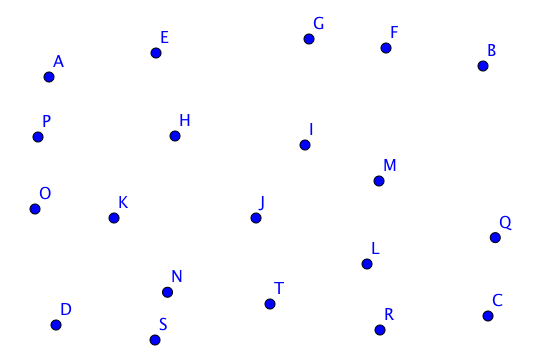
\includegraphics[width=\linewidth]{set_of_points}
\caption{Set of points}\label{fig:points}
\end{subfigure}\hspace{20 mm}
\begin{subfigure}[b]{.33\linewidth}
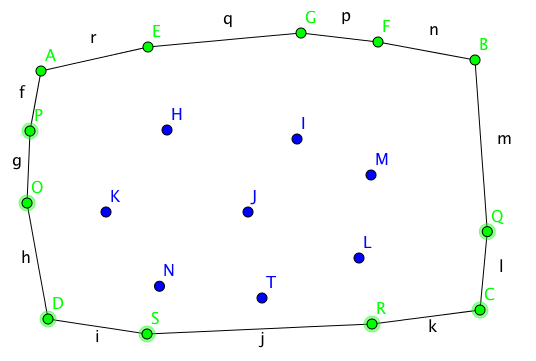
\includegraphics[width=\linewidth]{convex_hull_of_set}
\caption{Convex hull in green}\label{fig:convex_hull}
\end{subfigure}\hspace{20 mm}
\begin{subfigure}[b]{.33\linewidth}
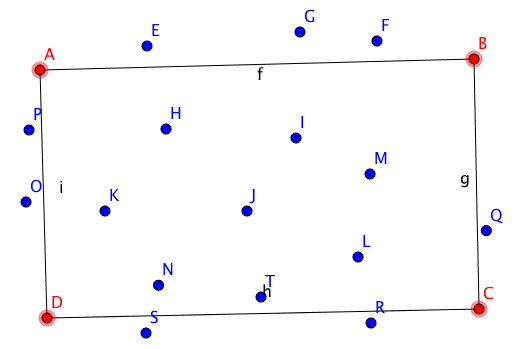
\includegraphics[width=\linewidth]{approximate_convex_hull}
\caption{Approx convex hull in red}\label{fig:approx_convex_hull}
\end{subfigure}
\caption{Convex hull and approximate convex hull of a set of points.}
\label{fig:hull_overview}
\end{figure}

Intuitively, an optimal convex hull captures the boundary of a set of points. Figure~\ref{fig:points} shows a set of points, and figure~\ref{fig:convex_hull} shows an optimal convex hull of the points. 

\section{Approximate Convex Hulls}

In many cases, we do not need to capture the boundary of a point set exactly - it suffices to have an approximation. For example, figure~\ref{fig:approx_convex_hull} highlights a smaller set of points that approximately captures the set of points. In particular, every point is either inside the approximate convex hull, or almost inside (within some distance $\epsilon$) the approximate convex hull. In these cases it is wasteful to store the entire convex hull, we can often store far fewer points and achieve a good enough approximation. We formalize these ideas with some definitions.

\begin{definition}
Given a set of points $S \subseteq \mathbb{R}^n$, we say that $p$ is an \emph{$\epsilon$-approximate convex combination} of $S$ if there exists some convex combination $q$ of points in $S$ with $|p - q|_2 \leq \epsilon$.
\end{definition}

\begin{definition}
Given a set of points $P \subseteq \mathbb{R}^n$, $S \subseteq P$ is an \emph{$\epsilon$-approximate convex hull} of $P$ if every $p \in P$ can be represented as an $\epsilon$-approximate convex combination of points in $S$. Importantly, \emph{an approximate convex hull of $P$ is made up of points in $P$}.
\end{definition}

If we don't restrict the approximate convex hull $S$ to come from the points in $P$, we can always choose 3 points that form a large triangle containing the points in $P$. However, this will typically not approximate the boundary of the original point set $P$. In Chapter~\ref{chapter:related_work} we examine some related problems where the approximate convex hull does not have to be made up of points in $P$.

\begin{figure}[!htb]
\centering
\begin{subfigure}[b]{.4\linewidth}
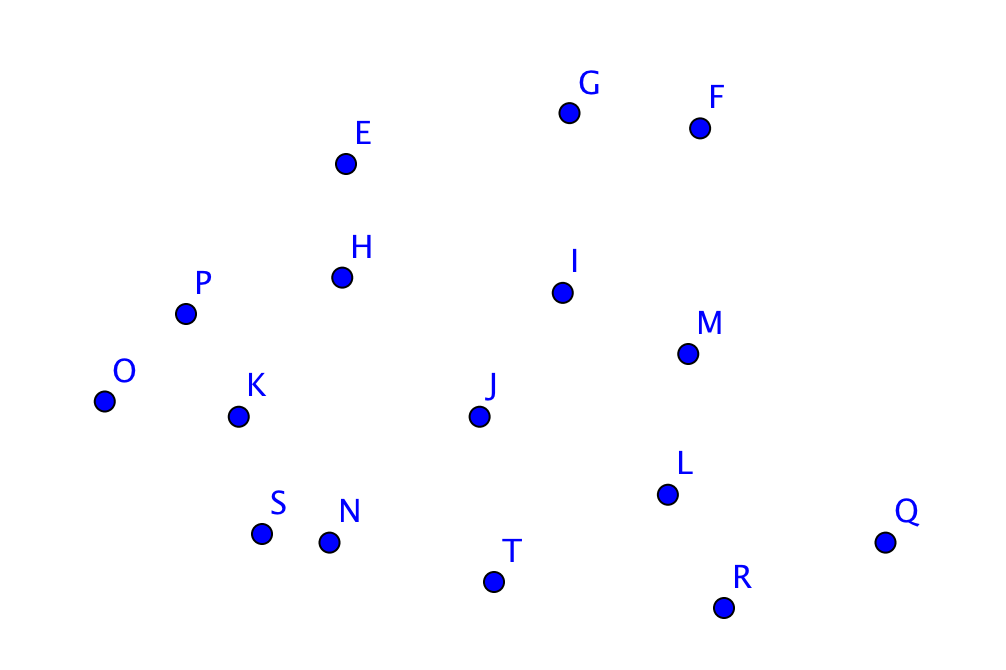
\includegraphics[width=\linewidth]{set_of_points_for_triangle}
\caption{Set of points}\label{fig:set_of_points_for_triangle}
\end{subfigure}\hspace{20 mm}
\begin{subfigure}[b]{.4\linewidth}
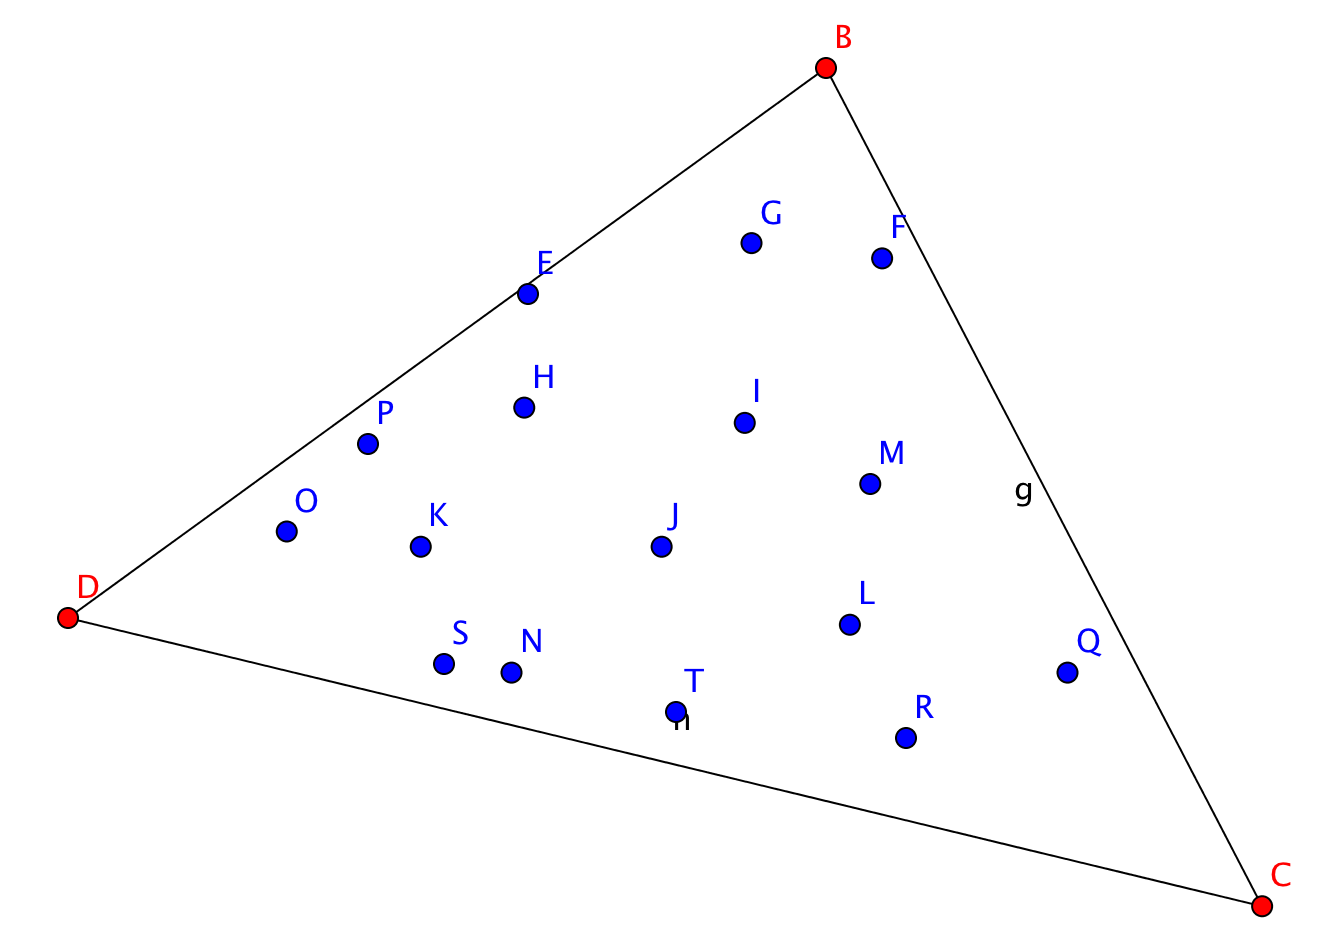
\includegraphics[width=\linewidth]{triangle_containing_set_of_points}
\caption{Triangle containing set of points}\label{fig:triangle_containing_set_of_points}
\end{subfigure}
\label{fig:triangle_containing_points}
\end{figure}

\begin{definition}
Let OPT$(P, \epsilon)$ denote the size of a (not necessarily unique) smallest $\epsilon$-approximate convex hull of $P$.
\end{definition}

\section{Batch vs Streaming}

A batch algorithm for the $\epsilon$-approximate convex hull problem takes a point set $P$, performs some sequence of operations, and outputs an $\epsilon$-approximate convex hull that is close in size to OPT$(P, \epsilon)$. In many cases, however, $P$ is too large to fit in memory.
\\

To address this, a streaming algorithm is only allowed to see each point once. After it sees the entire point set $P$, it outputs an $\epsilon$-approximate convex hull that is close in size to OPT$(P, \epsilon)$. Streaming algorithms are used in contexts where $P$ is too large to fit in memory, and are therefore assessed on the amount of memory that they use. Ideally, a streaming algorithm would use space close to OPT$(P, \epsilon)$, where $P$ is the set of points it has processed so far. Although the runtime of streaming algorithms is also important, we focus on the space complexity of streaming algorithms.
\\

We often distinguish between a set of points and a stream of points. A set of points is unordered, while a stream of points is ordered and might even contain duplicates of the same point (at different locations in the ordering).

\section{Contributions}
\label{sec:contributions}

The main aim of this thesis is to come up with good streaming algorithms for finding $\epsilon$-approximate convex hulls. We show some lower bounds to justify that this is a hard problem. In particular, we show that under a reasonable streaming model it is not possible for a streaming algorithm to be competitive with OPT (in fact, an arbtirary function of OPT) in 3D or higher. This implies that we need to relax the problem or the streaming model, or the space bound needs to include some function of $\epsilon$ or $n$ (the size of the point set).
\\

We devise and prove streaming algorithms for two relaxations of the problem. In the first relaxation, the points are on a 2D plane and come in a random order. Our algorithm maintains an initially empty point set $S$. When our algorithm sees a new point $p$, it adds $p$ to $S$ if $p$ is at least distance $\epsilon$ away from the convex closure of $S$. Additionally, our algorithm keeps removing points $p \in S$ where $p$ is contained inside the convex hull of $S \setminus \{ p \}$, that is, removing $p$ does not change the convex hull of $S$. Surprisingly, for any point stream $P$, with high probability this algorithm keeps OPT$(P, \epsilon) \log{n}$ points, where $n$ is the size of $P$.
\\

In the second relaxation, the points come in an arbitrary order in $d$-dimensional space, but we only need to be correct in ``most" directions (all but a $\delta$ fraction of directions). Our algorithm picks $O(\frac{k^2}{\delta^2}\log{\frac{k}{\delta}})$ random unit vectors, where $k = \mbox{OPT}(P, \epsilon)$. For each of these vectors $v$, we keep the point in the stream that has maximal dot product with $v$. We give a proof based on VC-dimension to show that this algorithm achieves the desired bound. For 2D we achieve an even stronger bound.
\\

Both our algorithms are simple, and we find the fact that they achieve these bounds to be surprising. These algorithms and their proofs are the core contributions of this work.
\\

Another contribution of our work is to explain some of the connections between coresets, non-negative matrix factorization, and $\epsilon$-approximate convex hulls, and their limitations. We give some experimental evidence for the connection between non-negative matrix factorization and our notion of approximate convex hulls.
\\

There has been lots of recent work on $\epsilon$-approximate convex hulls, and even streaming $\epsilon$-approximate convex hulls. However, to our knowledge, this is the first work that examines streaming algorithms for $\epsilon$-approximate convex hulls in relation to the optimal, that is, OPT$(P, \epsilon)$.


\chapter{Background and Related Work}
\label{chapter:related_work}

% I scanned through a lot of the cites quickly, but I might have made mistakes while describing their results. I've commented on specific papers that I had a bit of trouble understanding, and we'd have to take a closer look in the final draft.

Approximate convex hulls are very useful because they give a good estimate of the boundary of a set of points, often using much less space than the true convex hull. In most cases where the true convex hull is used, we can tolerate some error, and so we can use an approximation instead. Direct applications of such boundary approximations include surface simplification~\cite{Heckbert97surveyof}, but they also play an important role in coresets and non-negative matrix factorization.
% Check the surface simplification reference more carefully, it seems to be true, but

\section{Coresets}

Given a set of points $P \subseteq \mathbb{R}^n$, we might be interested in some property of the set, $\mu(P)$. For example, we might want to know the volume of the smallest sphere containing $P$. More precisely, $\mu$ is a map from $\mathbb{R}^n$ to $\mathbb{R}^+ \cup \{0\}$, and is monotone, that is, if $P_1 \subseteq P_2$ then $\mu(P_1) \leq \mu(P_2)$.

\begin{definition}
An $\epsilon$-coreset~\cite{Agarwal:2004:AEM:1008731.1008736,survey}, $S \subseteq P$ gives us an approximation of $\mu(P)$, where $\epsilon > 0$. In particular, $(1-\epsilon)\mu(P) \leq \mu(S) \leq \mu(P)$. 
\end{definition}

The general principles behind coresets are used in machine learning~\cite{cvms, peled-application, Feldman:2011:STM:2986459.2986698, Feldman, icml2015_bachem15}, robotics~\cite{6907021}, clustering~\cite{Har-Peled:2004:CKK:1007352.1007400}, and many other areas of research.

\subsection{$\epsilon$-kernels}

One of the most important types of coresets is the $\epsilon$-kernel~\cite{Agarwal:2004:AEM:1008731.1008736,survey}, because it is a coreset for many properties $\mu$.

\begin{definition}
Given a set of points $P \subseteq \mathbb{R}^d$ and $u \in \mathbb{R}^d$ with $|u|_2 = 1$, the \emph{directional width} of $P$ in direction $u$ is given by,
\[ \omega(u, P) = \max_{p \in P}\langle p, v \rangle - \min_{p \in P}\langle p, v \rangle \] 
\end{definition}

\begin{definition}
A subset $Q$ of $P$ is called an $\epsilon$-kernel of $P$ if for all $u$ with $|u|_2 = 1$,
\[ (1 - \epsilon) \omega(u, P) \leq \omega(u, Q) \]
\end{definition}

In both the batch and streaming setting, algorithms to find an $\epsilon$-kernel almost always reduce to finding an $\epsilon$-approximate convex hull of a set of points contained in the unit sphere. Most of these algorithms also assume that the dimension $d$ is a constant (so even a $d^d$ multiplicative term in the time or space complexity is ignored).
\\

$\epsilon$-kernels are used in a wide range of applications. For example, Barequet and Har-Peled~\cite{BAREQUET200191} explain how $\epsilon$-kernels can be used to efficiently approximate the minimum volume bounding box containing a set of points. Minimum volume bounding boxes are used in computer graphics (for fast scene rendering and collision detection), and statistics (for range queries on samples)~\cite{BAREQUET200191}. Agarwal, Har-Peled, and Varadarajan~\cite{Agarwal:2004:AEM:1008731.1008736} explain how $\epsilon$-kernels can also be used to find the minimum width cylinderical shell, and the minimum width sphere, containing a set of points. $\epsilon$-kernels can also be used to approximate k-regret minimizing sets~\cite{DBLP:journals/corr/AgarwalKSS17}.

\subsection{Batch Algorithms for $\epsilon$-kernels}

In the batch setting, Bentley, Preparata, and Faust~\cite{Bentley:1982:AAC:358315.358392} give a $1/\epsilon^{d-1}$ space algorithm for computing an $\epsilon$-approximate convex hull of a set of points. Agarwal, Har-Peled, and Varadarajan~\cite{Agarwal:2004:AEM:1008731.1008736} use this to give a $1/\epsilon^{d-1}$ space algorithm for computing an $\epsilon$-kernel. This was improved to a $1/\epsilon^{\frac{d-1}{2}}$ space algorithm~\cite{Yu:2004:PMS:997817.997858, CHAN200620} for computing an $\epsilon$-kernel. The time bounds on these algorithms were further improved~\cite{timchansocg2017, aryasocg2017}. All of these methods involve computing the $\epsilon$-approximate convex hull.
\\
% Confirm that Agarwal, Har-Peled, and Varadarajan's original algorithm is 1/eps^(d-1) and not 1/eps^((d-1)/2)
% Cinfirm that all timchansocg2017 and aryasocg2017 did was improve the time bound, and not the space bound.

Ignoring specific details about the point set $P$, the space usage of $1/\epsilon^{\frac{d-1}{2}}$ is optimal: there exists some set of points $P$ where the $\epsilon$-approximate convex hull (and the $\epsilon$-kernel) must store $1/\epsilon^{\frac{d-1}{2}}$ points.
\\

However, in many cases, the $\epsilon$-approximate convex hull is much smaller than $1/\epsilon^{\frac{d-1}{2}}$. For example, suppose we have points $p_1, p_2, p_3$ in high dimensional space. We generate data points by taking convex combinations of $p_1, p_2, p_3$, and then perturbing the generated point by $\epsilon$. Suppose we give the algorithm a set of points $P$ containing $p_1, p_2, p_3$ and the generated data points. The $\epsilon$-approximate convex hull of this set has size at most 3 (it suffices to keep $p_1, p_2, p_3$), and it would be wasteful to store $1/\epsilon^{\frac{d-1}{2}}$ points especially when $d$ is large. Blum, Har-Peled, and Raichel~\cite{blum-peled} give the only known algorithms for $\epsilon$-approximate convex hulls that are competitive with the optimal of the given point set.

\subsection{Streaming Algorithms for $\epsilon$-kernels}

In many cases, the point set might be much larger than the amount of memory available (for example in financial markets, packet flow monitors, sensor networks)~\cite{Hershberger:2004:ASG:1055558.1055595}. In these cases we want a streaming (one pass) algorithm that sees each point exactly once, and has low memory consumption.
\\

Hershberger and Suri give a 2D streaming algorithm for $\epsilon$-approximate convex hulls that uses $1/\sqrt{\epsilon}$ space~\cite{Hershberger:2004:ASG:1055558.1055595}. Agarwal, Har-Peled, and Varadarajan~\cite{Agarwal:2004:AEM:1008731.1008736} give a streaming algorithm for $\epsilon$-kernels that uses $(1/\epsilon^{\frac{d-1}{2}})\log^d{n}$ space. Chan removes the dependency on $n$ and gives a streaming algorithm for $\epsilon$-kernels that uses $(1/\epsilon^{d-3/2})\log^d{1/\epsilon}$ space~\cite{CHAN200620}. This was then improved to $(1/\epsilon^{\frac{d-1}{2}})\log{1/\epsilon}$~\cite{Zarrabi-Zadeh:2011:ASS:1967334.1967341} and the time complexity was further improved by Arya and Chan~\cite{Arya:2014:BOA:2582112.2582161}. Chan also gives a streamling algorithm based on polynomial methods~\cite{chansocg2016}. All of these methods involve clever tricks and transformations, but a core part of these methods is a streaming algorithm to maintain an $\epsilon$-approximate convex hull of a set of points.
\\
% How is Agarwal, Har-Peled, and Varadarajan's streaming algorithm 1/eps^((d-1)/2), something is fishy.

Like in the batch case, if we ignore the particular point set $P$ we are dealing with, a space usage of $\frac{1}{\epsilon^{(d-1)/2}}$ is optimal. However, in many cases we can do much better. In this work our aim is to come up with streaming algorithms that are competitive with the optimal $\epsilon$-approximate convex hull of the given point set. To our knowledge there is no existing work of this kind.

\section{Matrix Factorization}

Matrix factorization is a popular technique in unsupervised machine learning.

\subsection{Non-Negative Matrix Factorization (NMF)}

In classical non-negative matrix factorization (NMF) we are given $n$ data points, with non-negative coordinates, in $d$ dimensional space. We want to find a minimal collection $T$ of topics with non-negative coordinates such that every data point can be represented as a non-negative linear combination of the topics in $T$. In approximate non-negative matrix factorization the data points should be approximately representable (based on some distance metric) as a non-negative linear combination of the topics in $T$. 
\\

Non-negative matrix factorization decomposes objects into parts comprising those objects. For example, Lee and Seung use NMF ~\cite{leeseung95} to represent images of faces as combinations of parts in those faces, as shown in figure~\ref{fig:image-nmf}.

\begin{figure}[!ht]
\centering
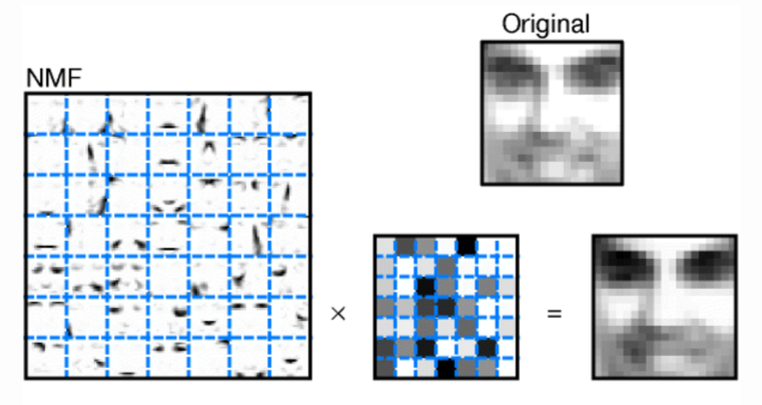
\includegraphics[scale=0.3]{image-nmf}
\caption{The boxes on the left represent parts of the face that are summed together to approximate the face}
\label{fig:image-nmf}
\end{figure}

Lee and Seung also used NMF to find out what topics encyclopedic articles are about ~\cite{leeseung95}. For example, the encyclopedic entry `constitution of the United States' was decomposed into a topic represented by the words (`court', `government', `council', `culture', `supreme', ...) and a topic represented by the words (`president', `served', `governer', `secretary', `senate', ...). NMF has a wide range of applications. For example, NMF is used for text mining~\cite{Berry2005, Murphy2012LearningEA}, speech de-noising~\cite{schmidt-noise}, and energy disaggregation~\cite{Kolter:2010:EDV:2997189.2997318}.
\\

Related matrix factorization methods, like PCA, allow negative weights. While PCA has many important uses, NMF gives a better parts based decomposition~\cite{leeseung95}. This is because a lot of data, like audio signals, is built up from a non-negative sum of of signals, for example we might add the sound of birds chirping to the sound of leaves rustling in the wind. Allowing negative weights could lead to complex cancellations which lead to a less intuitive representation. For example, natural audio signals do not typically involve subtracting the sound of birds chirping, and images of faces do not involve subtracting a nose from a face.

\subsection{Algorithms for NMF}

Stated more formally, in NMF we are given a $d-$by$-n$ matrix $A$ where the columns are data points. We want to find the smallest $d-$by$-t$ topic matrix $T$ where the columns represent topics, and a $t-$by$-n$ weights matrix $W$ where the columns represent weights s.t. $A = TW$. In some formulations~\cite{leeseung95}, entries of $A$, $T$, and $W$ are non-negative, in some formulations only the weights matrix $W$ is required to be non-negatvie~\cite{NIPS2016_6417}. In approximate NMF, we are given a distance metric $d$ and a distance $\epsilon$ and want to find the smallest $T$ s.t. $d(A,TW) < \epsilon$. Alternatively, we are given $k$ and a norm $|\cdot|$, and want to minimize $|A-TW|$, where $T$ has $k$ columns.
\\

NMF is NP-complete ~\cite{nmf-np-complete}, so most approaches focus on finding approximation algorithms or solving NMF for certain classes of problems. Lee and Seung use a multiplicative update rule and show that their approach converges to a local optimum ~\cite{Lee00algorithmsfor}. Alternatively, it can be shown for common distance metrics that the optimization problem is convex if we fix $T$ or $W$. Lin uses this to alternate between optimizing $T$ and $W$ using gradient descent, and shows that this converges to a local optimum ~\cite{lin-grad-optimization}. 
\\

Donoho and Stodden introduce a condition called separability~\cite{NIPS2003_2463}: $A$ is separable if each column contains some row which is $1$ only in that column. For example, if each article in a collection has an `anchor' word that is unique to the article then the collection is separable. Arora et al prove an efficient polynomial time algorithm for separable NMF ~\cite{DBLP:arora} and show that separable NMF works well in practice~\cite{DBLP:arora-practice}. More recent research focuses on near separability~\cite{Gillis:2014:RNN:2627435.2638575}.

\subsection{Sparse Coding}

 The number of topics is often large. Instead of simply finding the smallest topic matrix $T$ such that $A = TW$, we might want to find $T$ so that every data point can be represented (or approximately represented) as the sum of a small number of topics (for example, at most $k$ topics). This problem is known as \emph{sparse NMF} or \emph{non-negative sparse coding}. Clustering requires every data point to be approximately represented by exactly one topic in $T$.
 \\
 
Intuitively, sparsity is appealing because objects tend to be made up of a small number of parts. Another way of looking at this is that without sparsity, we might overfit the topics to the data. In particular, if we have $n >> d$ points in $d$ dimensional space, we can simply pick a unit vector along each axis as our topics. Every data point can be represented as a non-negative combination of these vectors, but this representation does not reveal any structure about the data.
\\

In some cases, NMF naturally gives a sparse representation. Lee and Seung show that NMF learns a sparse representation of facial images~\cite{leeseung95}. A combinatorial analogy for this is: suppose a human face is built up from a sum of 5 different types of noses, 5 different types of eyes, and 5 different types of mouths. There are 125 possible faces, which represent combinations of these parts. A non-negative matrix factorization with 15 topics is forced to learn the 5 noses, 5 eyes, and 5 mouths that add up to the face in order to give a compact representation.
\\

However, in some cases NMF does not give a meaningful or sparse representation, and the degree of sparsity in NMF cannot be tuned~\cite{hoyer-nmf}. Sparse NMF, which is related to sparse coding, adds additional constraints to incentivize sparsity. Many algorithms for sparse NMF simply use $L_1$ or $L_2$ regularization on the weights matrix $W$~\cite{Lee97unsupervisedlearning, Berry2005, Mairal:2010:OLM:1756006.1756008, Murphy2012LearningEA}. There has been a lot of research on sparse NMF. Hoyer gives an algorithm for sparse NMF and shows that it performs well on an image database~\cite{hoyer-nmf}. Schmidt, Larsen, and Hsiao use sparse NMF to separate wind noise from audio tracks~\cite{schmidt-noise}. 

\subsection{The Approximate Convex Hull Approach}

It turns out that $\epsilon$-approximate convex hulls can be used for sparse NMF~\cite{blum-peled}. In particular, suppose we normalize the columns of $A$ so that they lie in the unit sphere (for example by normalizing the $L_1$ or $L_2$ norm of each column to be 1). Let $T$ be a matrix where the columns correspond to an $\epsilon$-approximate convex hull (of the columns of $A$) of minimal size. Then, for all columns $A_i$ in $A$, there exists a convex combination $w$ such that $|A_i - Tw|_2 \leq \epsilon$. So this gives us a non-negative matrix factorization (on a different norm).
\\

Furthermore, we get a sparsity guarantee. In particular, for all culumns $A_i$ in $A$, there exists a convex combination $w$ with at most $1/\epsilon^2$ non-zero elements such that $|A_i - Tw|_2 \leq 2\epsilon$~\cite{Har-Peled:2016:SEV:2984951.2984998, blum-peled}.
\\

The hyperspectral unmixing literature often works with non-negative matrix factorizations where the data points are scaled to have the same $L_1$ norm, and the weights are restricted to be convex. However, the topics are usually not restricted to come from the data points, their algorithms typically ensure that the topics form a simplex, and they use different error measures and regularization functions~\cite{6200362, gillis_survey}. More experiments would need to be done to see if our approch can be used for hyperspectral unmixing.
\\
% Verify that the hyperspectral unmixing paper scales to L1 norm. Their figures strongly suggest this, but they don't describe this.

Arora, Ge, Kannan, and Moitra, also scale the data points to have the unit $L_1$ norm. They explain that if we do this scaling then without loss of generality we can assume the weights are convex~\cite{Arora:2012:CNM:2213977.2213994, moitramonograph}. Lee and Seung suggest using convex weights and show that this gives better results in a USPS digit classification dataset, however in reality they use $L_2$ regularization to approximate the convexity constraint~\cite{Lee97unsupervisedlearning}. The main difference between these models and ours is that they use the Frobenius norm, whereas we ensure that all data points are within distance $\epsilon$ from the approximate convex hull. We might get more provable guarantees because of our stronger requirement, but our algorithms might be more sensitive to noise or might need a preprocessing step to get rid of noise. Additionally, we restrict our topics to be data points (that is, each column of $T$ is a column of $A$).
\\

We follow the experimental setup in~\cite{Lee97unsupervisedlearning} to test the assumptions of our model. We use the MNIST classification task. Our preliminary experiments (see Appendix A) show that for large topic matrices, using an approximation algorithm to find an $\epsilon$-approximate convex hull (described in~\cite{blum-peled}) outperforms using Matlab's non-negative matrix factorization method. While these experiments are not thorough, they suggest that our modeling differences from other papers in the NMF literature might be reasonable.



\chapter{Streaming Model and Lower Bounds}
\label{chapter:lower_bounds}
We prove lower bounds to show that coming up with good streaming algorithms for approximate convex hulls is difficult.

\section{Streaming Model}

Given a stream/sequence of points $P$. A streaming algorithm $A$ is given $\epsilon$ in advance but is not given the size of the point stream $P$. As $A$ processes $P$ it maintains a subset $S$ of the points it has seen so far.
\\

The streaming algorithm $A$ is given the points in $P$ sequentially. Each time $A$ is given a point $p \in P$, $A$ can choose to add $p$ to $S$ (remembering $p$) or ignore $p$ (and permanently forget $p$). $A$ can also choose to delete points in $S$, in which case these points are permanently lost. The important part is that $A$ cannot go back in time and access points it did not keep.
\\

Typically we want $S$ to be an $\epsilon$-approximate convex hull of the points seen so far. A trivial streaming algorithm could just keep all points it has seen so far. However, this is very wasteful since the assumption is that $P$ is too large to fit in memory. Our aim is for $A$ to be competitive with OPT.

% Given a sequence of points $P$ ordered from 1 to $n$, let $P_{i:j}$ denote the subsequence of points from index $i$ to $j$, inclusive of both indices.
% 
% 

\section{Always OPT Lower Bounds}

Consider a set of points $P$, and $S \subseteq P$. We begin by noting that OPT$(S, \epsilon)$ could be a lot larger than OPT$(P, \epsilon)$. For example, setting $\epsilon = 0$, figure 1a shows the convex hull of a set of points, and figure 1b shows the convex hull of a subset of points. In particular, the number of points a streaming algorithm stores is not monotone. This simple fact gives us a trivial lower bound. Given a point stream $P$, it is impossible for a streaming algorithm to always maintain an $\epsilon$-approximate convex hull of the points it has seen so far, that is competitive in size with OPT$(P, \epsilon)$. This is because the $\epsilon$-approximate convex hull of the first half of stream $P$ can be arbitrarily larger than OPT$(P, \epsilon)$. We now move on to proving a much more interesting lower bound.
\\

\begin{definition}
For $r \in \mathbb{Z}^+$, we say a streaming algorithm $A$ is \emph{always-$r$-OPT} if there exists a function $f : \mathbb{Z}^+ \to \mathbb{Z}^+$ such that: if $A$ is run on an arbitrary point stream $P$, then after processing all points in $P$, $A$ keeps an $r\epsilon$-approximate convex hull of $P$ with size at most $f(\mbox{OPT}(P, \epsilon))$.
\end{definition}

Note that since the size of $P$ was not given to $A$ in advance, this property holds for all prefixes of $P$ as well. In particular, for every prefix $T$ of $P$, the size of the $r\epsilon$-approximate convex hull $A$ stores after seeing all the points in $T$ is at most $f(\mbox{OPT}(T, \epsilon))$. Intuitively, when an always-$r$-OPT algorithm is run on a stream, it always maintains an $r\epsilon$-approximate convex hull that is competitive with the optimal of the points seen so far.

\begin{definition}
We say a point $p$ is interior to $P$ if $p$ is in the convex hull of $P \setminus \{p\}$.
\end{definition}

\begin{definition}
We say a set of points $P$ is \emph{meaningful} if $P$ has no interior points. Alternatively, the optimal convex hull of $P$ is $P$.
\end{definition}

\begin{definition}
For $\epsilon > 0$, we say a set of points $P$ is \emph{$\epsilon$-meaningful} if the optimal $\epsilon$-convex hull of $P$ is $P$. This means the distance from point $p \in P$ to the convex hull of $P \setminus \{p\}$ is at least $\epsilon$.
\end{definition}

\begin{lemma}
If $P$ is $\epsilon$-meaningful then $P$ is meaningful. In the other direction, if $P$ is meaningful then there exists $\epsilon > 0$ such that $P$ is $\epsilon$-meaningful.
\end{lemma}

\begin{theorem}
There does not exist an always-1-OPT streaming algorithm in 3D.
\label{thm:alwaysopt}
\end{theorem}

\begin{proof}
Assume for the sake of contradiction that there exists some always-1-OPT streaming algorithm $A$ and corresponding function $f : \mathbb{Z}^+ \to \mathbb{Z}^+$. Without loss of generality, we can assume that $f$ is increasing.
\\

The high level idea is that we will construct 3 sequences of points $P_1$, $P_2$, $P_3$. Let $P_1 @ P_2$ denote sequence $P_1$ followed by sequence $P_2$. We will show that if $A$ keeps an $\epsilon$-approximate convex hull of size at most $f(\mbox{OPT}(P_1 @ P_2, \epsilon))$ after receiving $P_1 @ P_2$, then it cannot keep an $\epsilon$-approximate convex hull of size at most $f(\mbox{OPT}(P_1 @ P_2 @ P_3, \epsilon))$ after receiving $P_1 @ P_2 @ P_3$.
\\

All points in $P_1$ will have $z$-coordinate 0, all points in $P_2$ will have $z$-coordinate $\epsilon$, all points in $P_3$ will have $z$-coordinate $2\epsilon$, where $\epsilon$ will be specified later. Geometrically, one can visualize three planes perpendicular to the $z$ axis with points in $P_1$, $P_2$, $P_3$ on their respective planes. We now treat $P_1, P_2, P_3$ as point sets in 2D and specify the $x$ and $y$ coordinates of points in the sets.

\begin{figure}[!htb]
\centering
\begin{subfigure}[b]{.25\linewidth}
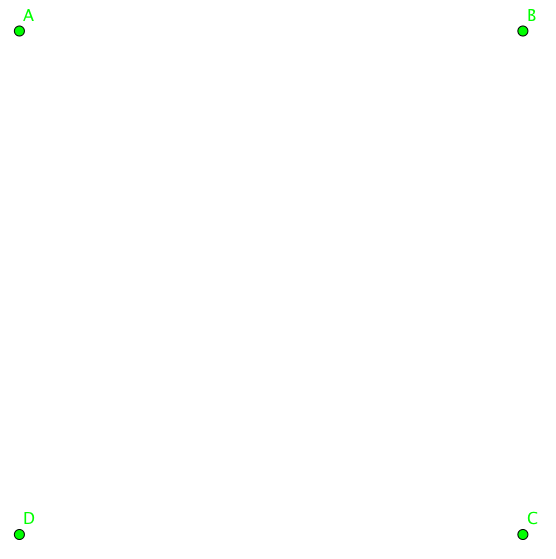
\includegraphics[width=\linewidth]{layer1square}
\caption{$P_1$ at $z=0$}\label{fig:layer1}
\end{subfigure}\hspace{10 mm}
\begin{subfigure}[b]{.25\linewidth}
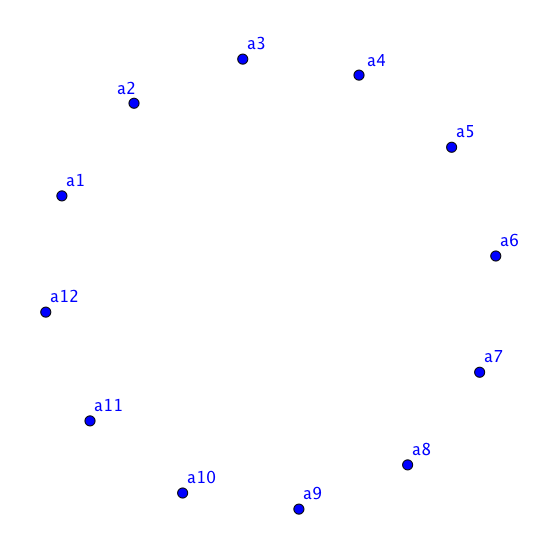
\includegraphics[width=\linewidth]{layer2regular}
\caption{$P_2$ at $z = \epsilon$}\label{fig:layer2}
\end{subfigure}\hspace{10 mm}
\begin{subfigure}[b]{.25\linewidth}
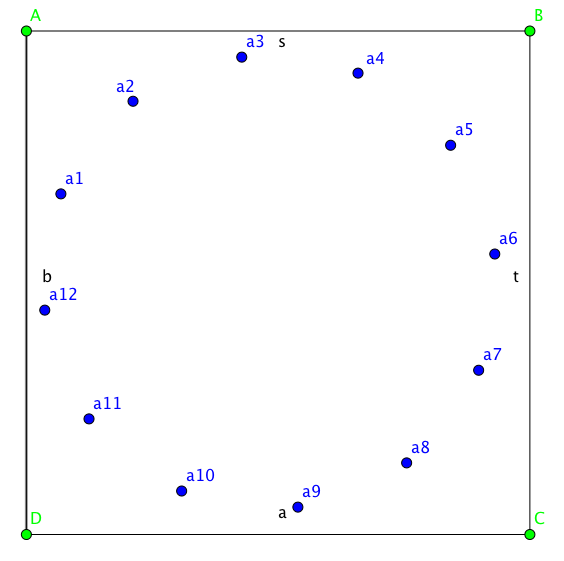
\includegraphics[width=\linewidth]{layer1and2}
\caption{$P_1, P_2$ projected}\label{fig:layer1and2}
\end{subfigure}
\caption{2D depiction of points in $P_1$ and $P_2$, ignoring $z$ coordinates}
\label{fig:lower_bound_construction_overview}
\end{figure}

$P_1$ contains 4 points that form a square, with coordinates, $(0,0)$, $(0,1)$, $(1, 0)$, $(1, 1)$, as shown in figure~\ref{fig:layer1}. $P_2$ has $n = 10f(4)$ points, forming a regular polygon that is centered around $(0.5, 0.5)$ with $x, y$ coordinates between 0 and 1, as shown in figure~\ref{fig:layer2}. So if we ignore the $z$ coordinates, $P_2$ is contained inside $P_1$, as shown in figure~\ref{fig:layer1and2}. Order the points in $P_2$ anti-clockwise, $a_1, ..., a_n$. Group the points into disjoint sets of 5 consecutive points. So the first group will have the points $a_1, ..., a_5$, the second group has the points $a_6, ..., a_{10}$, etc. For each group of 5 points in $P_2$ we will construct $m = 10f(n+4) = 10f(10f(4) + 4)$ points in $P_3$.

\begin{figure}[!htb]
\centering
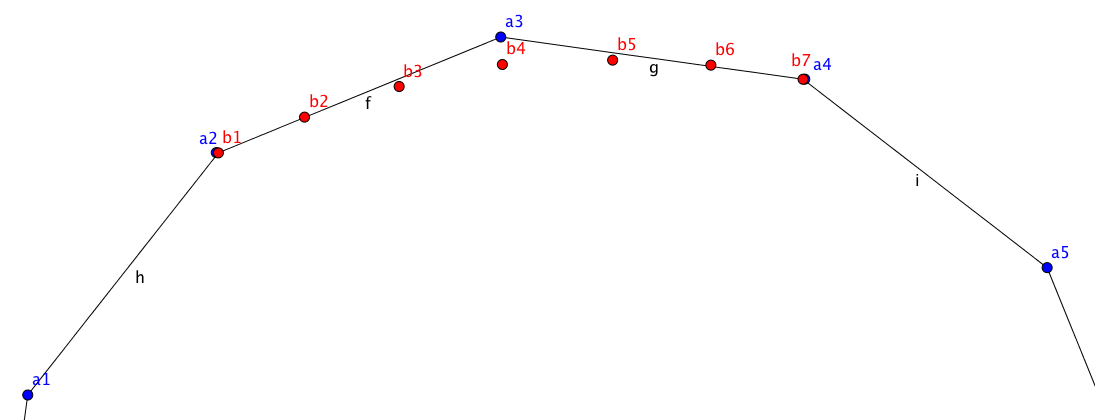
\includegraphics[width=0.6\linewidth]{layer3points}
\caption{Red points are in $P_3$, blue in $P_2$}
\label{fig:layer3}
\end{figure}

WLOG consider $a_1, ..., a_5$ in $P_2$. For each such group, we will add points $b_1, ..., b_m$ to $P_3$. Ignoring $z$ coordinates, we set $b_1 = a_2$, $b_m = a_4$. All the points $b_1, ..., b_m$ will be contained in the triangle defined by $a_2, a_3, a_4$. The points $b_1, ..., b_m$ are equally spaced, and form equal angles that are less than 180 degrees. We illustrate this construction in figure~\ref{fig:layer3}. We note that by our construction $P_1, P_2, P_3$ are meaningful. We choose the smallest $\epsilon$ such that $P_1, P_2, P_3$ are $\epsilon$ meaningful. Now, we will prove the theorem.
\\

Suppose we run $A$ on $P_1 @ P_2$. Ignoring $z$ coordinates, $P_2$ is contained inside $P_1$. Since the $z$ coordinates of points in $P_1$ and $P_2$ are $0$ and $\epsilon$ respectively, $P_1$ is an $\epsilon$-approximate convex hull for $P_1 @ P_2$. So OPT$(P_1 @ P_2, \epsilon) \leq 4$. Since $A$ is always-1-OPT, it can keep at most $f(4)$ points in $P_1 @ P_2$. $P_2$ has a total of $10f(4)$ points, which we divided into $2f(4)$ groups of $5$ points. So $A$ did not store any points in at least $f(4)$ of these groups, call these the unselected groups in $P_2$.
\\

Now suppose we run $A$ on $P_1 @ P_2 @ P_3$. For each of the $f(4)$ unselected groups in $P_2$, we selected $m = 10f(n+4)$ points in $P_3$. $A$ has to select all the corresponding $m$ points in $P_3$. To prove this, suppose for the sake of contradiction we don't have to select some corresponding point $p$ in $P_3$. $p$ cannot be written as an $\epsilon$-approximate convex combination of selected points in $P_2$, because the $z$ coordinate of $p$ and points in $P_2$ differ by $\epsilon$ \emph{and} if we ignore $z$ coordinates (projecting to the plane $z = 0$) $p$ corresponds to an unselected group and so does not lie inside the convex hull of selected points in $P_2$. Furthermore, since we selected $P_3$ to be $\epsilon$-meaningful, $p$ cannot be written as an $\epsilon$-approximate convex combination of other points in $P_3$.
\\

Summing over unselected groups, this means that $A$ must keep $f(4)m = 10f(4)f(n+4)$ points in $P_3$. The optimal approximate hull of $P_1 @ P_2 @ P_3$ is much smaller: we can simply store all the points in $P_1$ and $P_2$ giving us a total of $n + 4$ points. So OPT$(P_1 @ P_2 @ P_3, \epsilon) \leq n + 4$, which means $A$ is allowed to keep at most $f(n+4)$ points. $10f(4)f(n+4) > f(n+4)$ so we have a contradiction. 

\end{proof}

\begin{theorem}
For all $r \in \mathbb{Z}^+$, there does not exist an always-$r$-OPT streaming algorithm in $\mathbb{R}^3$.
\label{thm:alwaysropt}
\end{theorem}

\begin{proof}
The construction is similar to theorem~\ref{thm:alwaysopt}, with a few differences. Instead of constructing 3 sets of points $P_1, P_2, P_3$, we construct $r+1$ sets of points $P_1, ..., P_{r+1}$. All points in $P_i$ will have $z$ coordinate $(i-1)\epsilon$. For the $x, y$ coordinates, the construction of $P_{i+1}$ for $i \geq 2$ is similar to the construction of $P_3$ in theorem~\ref{thm:alwaysopt}. We group $P_i$ into disjoint groups of $5$ points. Let $n_i$ be the total number of points in $P_1, ..., P_i$. For each group in $P_i$ we add $10f(n_i)$ points in $P_{i+1}$. We then choose $\epsilon$ so that $P_i$ is $r\epsilon$ meaningful for all $i$.
\\

The proof of the construction is also similar to theorem~\ref{thm:alwaysopt}, except we apply the argument inductively. We can show that for each $i$, there exists an unselected group of 5 points in $P_i$, and further if we project onto $z=0$ the unselected group would be at least distance $r\epsilon$ outside the convex hull of points we select in $P_2, ..., P_{i-1}$. At $P_{r+1}$, this will give us an unselected point that is not an $r\epsilon$-approximate convex combination of selected points.
\end{proof}

\begin{corollary}
The above proof holds for both deterministic and randomized algorithms since it first presents a construction, and then cases on a particular run of the algorithm. It does not assume the algorithm runs the same way each time.
\end{corollary}

\begin{corollary}
For all $r \in \mathbb{Z}^+$ and $n \geq 3$, there does not exist an always-$r$-OPT streaming algorithm in $\mathbb{R}^n$.
\end{corollary}

\begin{proof}
If $n \geq 3$, $\mathbb{R}^n$ contains a 3D subspace so we can use the previous construction.
\end{proof}

% \section{Random Order Lower Bound}

% The 2D algorithm we give in chapter 4 works with high probability assuming that the points in the point stream come in a random order. In particular, every permutation of the stream $P$ must be equally likely. This assumption is very often true if the data is generated from a certain process (if the data points are i.i.d.). A natural question is whether assuming random order can give us an always-OPT streaming algorithm.

% \begin{definition}
% We say a streaming algorithm $A$ is \emph{weak random order always-OPT} if there exists $r \in \mathbb{Z}^+$ and a function $f : \mathbb{Z}^+ \to \mathbb{Z}^+$ such that: given an arbitrary point stream $P$, for at least 1\% of the permutations of $P$, if $A$ is run on the permutation, then after processing all points in $P$, $A$ keeps an $r\epsilon$-approximate convex hull of $P$ with size at most $f(\mbox{OPT}(P, \epsilon))$.
% \end{definition}

% \begin{theorem}
% For all $n \geq 3$, there does not exist a weak random order always-OPT streaming algorithm in $\mathbb{R}^n$.
% \end{theorem}

% \begin{proof}
% Filling it out now.
% % Given a point stream $P$ containing $n$ points ordered $p_1, ..., p_n$, we can essentially create a new point stream $P'$ that ``forces" the points to come in the same order as in $P$. Then we can use the construction in  }.
% % \\

% % We construct $P'$ inductively. For the base case, we will add 1 copy of the point $p_n$ to $P'$. For the inductive case, consider some $1 \leq i < n$. Suppose $P'$ currently has $m$ points (it only contains points $p_{i+1}, ..., p_n$ but it will contain multiple copies of most of these points). We will add $100nm$ copies of the point $p_i$ to $P'$.
% % \\

% % If $P'$ is randomly permuted, the probability that the first point in $P'$ is $p_1$ is $\geq 1 - \frac{1}{100n}$. So the probability that the first point is not $p_1$ is $\leq \frac{1}{100n}$. Intuitively, this is because most of the points in $P'$ are simply copies of $p_1$, so with very high probability we will see $p_1$ first. Continuing this process, and applying union bound, the probability the points do not come in the order $p_1, ..., p_n$ is at most $\frac{1}{100}$.
% % \\

% % So we can take the point stream $P_1 @ P_2 @ ... @ P_{r+1}$ we constructed in theorem~\ref{thm:alwaysropt} and apply this transformation to get a new point stream $P'$. For at least $\frac{99}{100}$ of the permutations of $P'$ the points will appear in the desired order
% % This means that for at least $\frac{99}$
% \end{proof}

\section{MAX-OPT Lower Bound}

We now show that even using a weaker notion of OPT, MAX-OPT, does not trivialize our problem.

\begin{definition}
Suppose that points in a point stream $P$ are ordered from 1 to $n$. Let $P_{i:j}$ denote a point stream containing the points from index $i$ to index $j$, inclusive of both index $i$ and $j$. In particular, $P_{1:n}$ is the entire point stream $P$.
\end{definition}

\begin{definition}
We define \emph{MAX-OPT$(P, \epsilon)$} as $\max_{1 \leq i \leq n} \mbox{OPT}(P_{i:n}, \epsilon)$, that is, the max of OPT taken over all prefixes of $P$.
\end{definition}

MAX-OPT is at least as large as OPT. Moreover, when we run an always-OPT algorithm $A$ on a stream $P$, at some point its memory usage must be a function of MAX-OPT. This is because MAX-OPT is OPT for some prefix $P'$ of $P$, and $A$ would have received the prefix $P'$ at some point. This is not too different from an algorithm that uses MAX-OPT space while processing the entire stream. The total (maximum) amount of memory we need to allocate to both algorithms is the same. So a natural question is whether a streaming algorithm can be competitive with MAX-OPT (independent of the number of points received so far). We define an always-MAX-OPT algorithm like an always-OPT algorithm, replacing OPT with MAX-OPT.

\begin{definition}
We say a streaming algorithm $A$ is \emph{always-MAX-OPT} if there exists $r \in \mathbb{Z}^+$ and a function $f : \mathbb{Z}^+ \to \mathbb{Z}^+$ such that: if $A$ is run on an arbitrary point stream $P$, then after processing all points in $P$, $A$ keeps an $r\epsilon$-approximate convex hull of $P$ with size at most $f(\mbox{MAX-OPT}(P, \epsilon))$.
\end{definition}

\begin{theorem}
For all $n \geq 3$, there does not exist an always-MAX-OPT streaming algorithm in $\mathbb{R}^n$.
\end{theorem}

\begin{proof}
The same construction and proof in theorem~\ref{thm:alwaysropt} works.
\end{proof}

\section{Almost Always OPT}

The algorithm we give in chapter 5 is of a slightly different nature.

\begin{definition}
A streaming algorithm $A$ is \emph{almost always OPT} if there exists a function $f : \mathbb{Z}^+ \to \mathbb{Z}^+$ such that the following holds. Suppose $A$ is given $k \in \mathbb{Z}^+$ in advance, and is run on an arbitrary point stream $P$ with $\mbox{OPT}(P, \epsilon) \leq k$. At any point, $A$ is allowed to keep at most $f(k)$ points. After processing all points in $P$, $A$ keeps an $\epsilon$-approximate convex hull of $P$.
\end{definition}

\begin{theorem}
There does not exist an almost always OPT streaming algorithm in $\mathbb{R}^3$.
\label{thm:almostalwaysopt}
\end{theorem}

\begin{proof}
We first prove this for a deterministic algorithm and then sketch out how to extend the proof to a randomized algorithm. Assume for the sake of contradiction that there exists a deterministic almost always OPT streaming algorithm in $\mathbb{R}^3$.
\\

We modify the construction in theorem~\ref{thm:alwaysopt}. We construct 3 points sets $P_1$, $P_2$, $P_3$. Points in $P_1, P_2, P_3$ have $z$-coordinates $0, \epsilon, 2\epsilon$ respectively, so we describe their $x, y$ coordinates. $P_1$ contains 4 points $(0,0), (0,1), (1,0), (1,1)$ like in theorem~\ref{thm:alwaysopt}. $P_2$ is a regular polygon centered around $(0.5, 0.5)$ with $x, y$ coordinates between $0$ and $1$. However, $P_2$ contains $n = 10f(7)$ points. We group the points in $P_2$ into consecutive groups of 5 like in theorem~\ref{thm:alwaysopt}.
\\

We will set $k=7$ and run $A$ on $P_1 @ P_2$. $A$ is allowed to keep at most $f(7)$ points, so it can keep at most $f(7)$ points in $P_2$. However, $P_2$ had $2f(7)$ groups of 5 points. So at least one of the groups is unselected, suppose the points in one of these groups are $a_1, ..., a_5$. For this group of 5 points, we use the construction we used in theorem~\ref{thm:alwaysopt} shown in figure~\ref{fig:layer3}, except we add $2f(7)$ (instead of $10f(10f(4) + 4)$) points to $P_3$. If we project all points onto the plane at $z = 0$ then $P_3$ will be contained inside the triangle defined by $a_2, a_3, a_4$.
\\

We define $\epsilon$ to be the smallest value such that $P_1, P_2, P_3$ are $\epsilon$-meaningful. Note that the choice of $\epsilon$ is independent of which group was unselected, since $P_2$ is a regular polygon and is therefore symmetric. Now, suppose we run $A$ on the stream $P_1 @ P_2 @ P_3$. $P_1 \cup \{ a_2, a_3, a_4 \}$ forms an $\epsilon$-approximate convex hull of $P_1 @ P_2 @ P_3$ so OPT$(P_1 @ P_2 @ P_3, \epsilon) \leq 7$. Since $A$ is almost always OPT, it must find a way to keep an $\epsilon$-approximate convex hull of $P_1 @ P_2 @ P_3$ of size $\leq f(7)$. However, $A$ must choose all points in $P_3$, because their distance from selected points in $P_1$ and $P_2$ is greater than $\epsilon$, and $P_3$ is $\epsilon$-meaningful. So $A$ must store $2f(7)$ points, a contradiction.
\\

This proof can be extended to show that there does not exist a randomized almost always OPT streaming algorithm in $\mathbb{R}^3$.
\end{proof}

Note that even if we use MOX-OPT instead of OPT, theorem~\ref{thm:almostalwaysopt} still holds.

\section{Limitations}

We believe that lower bounds should be treated as specific hardness results that guide research but that should not be generalized out of context or discourage work on a problem. The lower bounds we gave in this chapter have limitations, some of which are given below.

\begin{enumerate}
\item None of our lower bounds hold for 2D. Empirically, finding an always OPT or almost always OPT algorithm in 2D is a difficult problem, however it might not be impossible.
\item There might exist algorithms in higher dimensions that have a dependency on $\log{\frac{1}{\epsilon}}$ or $\log{n}$. For example we could be competitive with $\mbox{OPT} \cdot \log{\frac{1}{\epsilon}}$, which would still be a very useful result.
\item We could add reasonable assumptions, for example the assumption that the points come in a random order, which we do in chapter 4.
\item We might be able to relax the problem in useful ways and find solutions to those relaxations, like the relaxation we discuss in chapter 5.
\end{enumerate}


\chapter{Random Order Algorithm}

In this section we assume that the points are in 2D and come in a random order. In particular, for all sets of points $P$, every permutation of $P$ must have equal probability density.
\\

A special case of this is if the data points are generated from independent identical distributions. In this case, the probability density of a particular ordered point stream $P$ occuring can be factored into the product of the probability densities of each individual point occuring. Since multiplications can be reordered, this total probability is independent of the order in which the points occur.
\\

What makes the model powerful is that we are not making any assumptions about the distribution from which each individual point is generated, but simply that they are i.i.d. So this assumption would hold if the data points were generated from a mixture model, LDA, or even generalizations of these.
\\

\section{Algorithm Description}

Recall the definition of an interior point.

\begin{definition}
We say a point $p$ is interior to $P$ if $p$ is in the convex hull of $P \setminus \{p\}$.
\end{definition}

Our algorithm is simple. We begin by keeping a set $S = \{\}$. For each point $p \in P$ that the algorithm sees, if the distance from $p$ to the convex hull of $S$ is at most $\epsilon$, we discard $p$. Otherwise, we add $p$ to $S$. This is illustrated in figure 1: if the point $p$ is inside (figure~\ref{fig:point_inside_hull}) or near $S$ (figure~\ref{fig:point_slightly_outside_hull}) we discard $p$. Otherwise (figure~\ref{fig:point_far_outside_hull}) we add $p$ to $S$.
\\

\begin{figure}[!htb]
\centering
\begin{subfigure}[b]{.33\linewidth}
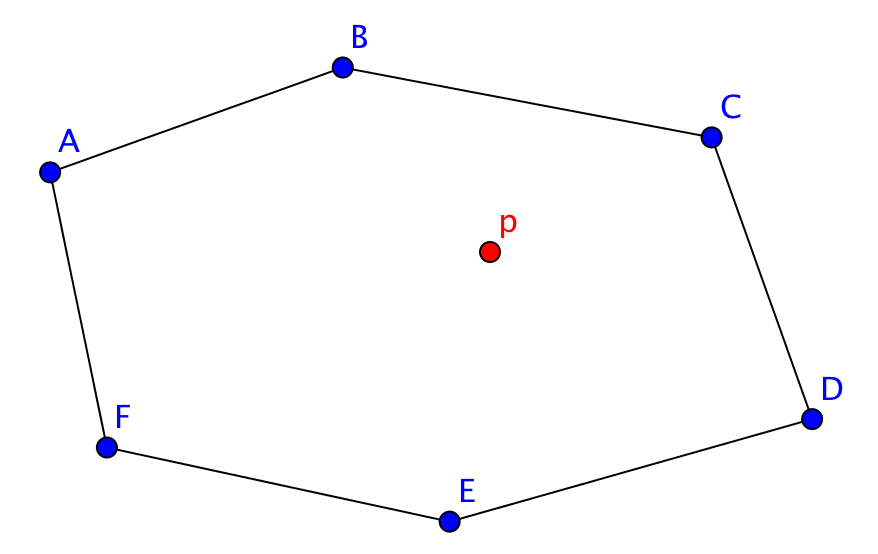
\includegraphics[width=\linewidth]{point_inside_hull}
\caption{Discard: $p$ inside hull}\label{fig:point_inside_hull}
\end{subfigure}\hspace{20 mm}
\begin{subfigure}[b]{.33\linewidth}
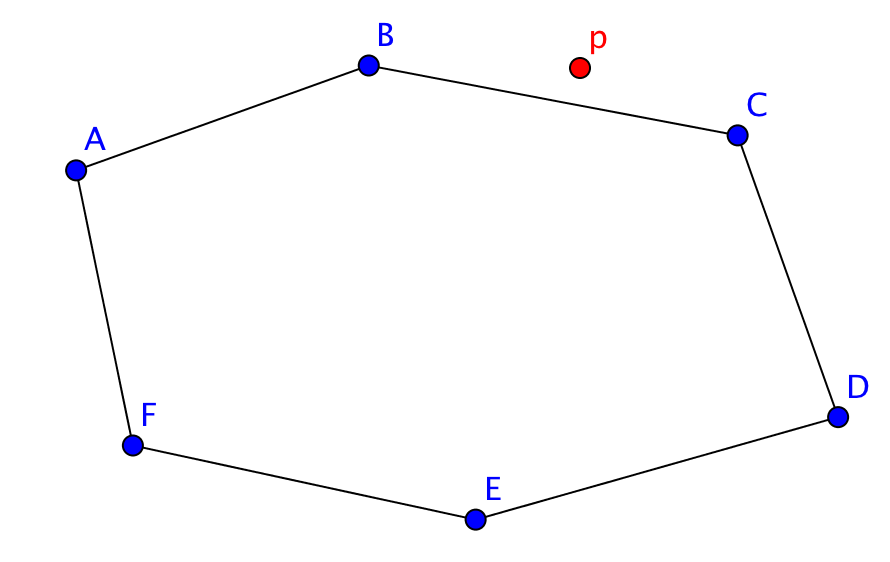
\includegraphics[width=\linewidth]{point_slightly_outside_hull}
\caption{Discard: $p$ near hull}\label{fig:point_slightly_outside_hull}
\end{subfigure}\hspace{20 mm}
\begin{subfigure}[b]{.33\linewidth}
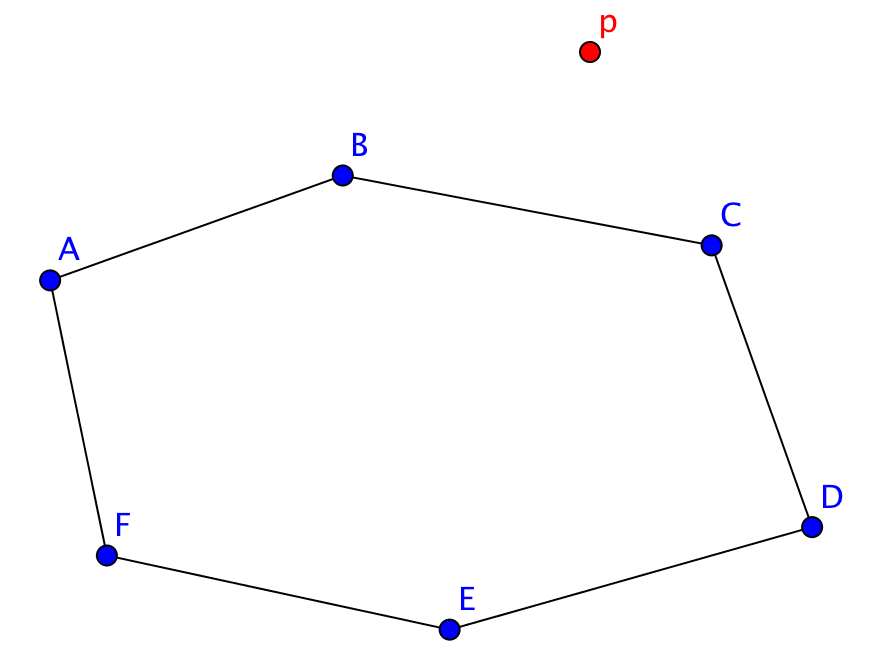
\includegraphics[width=\linewidth]{point_far_outside_hull}
\caption{Keep: $p$ far from hull}\label{fig:point_far_outside_hull}
\end{subfigure}
\caption{Our algorithm keeps point $p$ only if it is far from the current hull.}
\label{fig:when_to_discard_random_order}
\end{figure}

We then repeatedly delete interior points in $S$ until $S$ has no interior points. Figure~\ref{fig:2_interior_points} shows a point set with 2 interior points, and figure~\ref{fig:no_interior_points} shows the point set after removing all the interior points.
\\

\begin{figure}[!htb]
\centering
\begin{subfigure}[b]{.33\linewidth}
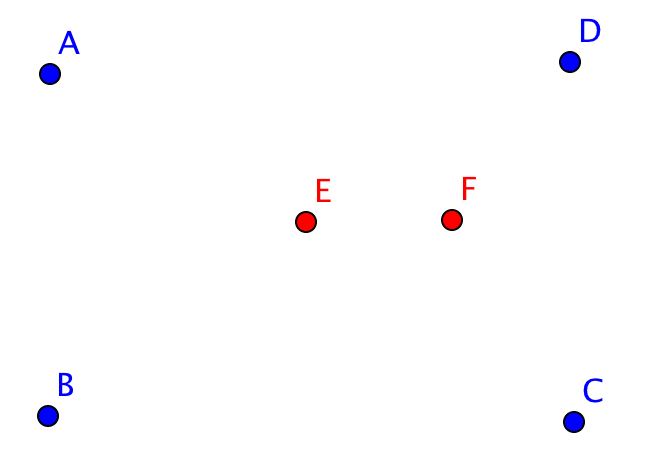
\includegraphics[width=\linewidth]{2_interior_points}
\caption{Interior points in red}\label{fig:2_interior_points}
\end{subfigure}\hspace{20 mm}
\begin{subfigure}[b]{.33\linewidth}
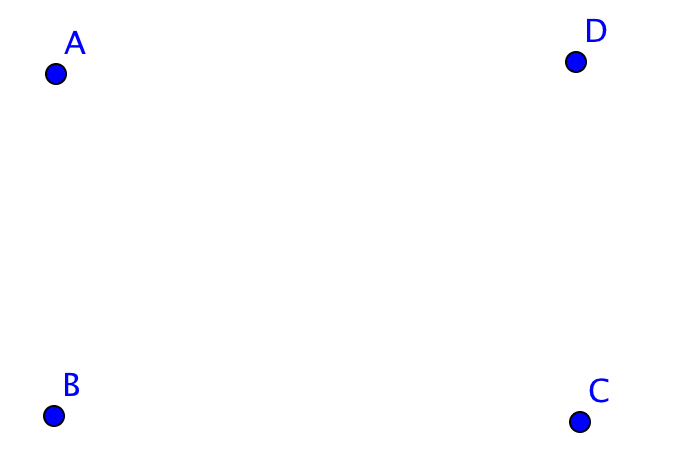
\includegraphics[width=\linewidth]{no_interior_points}
\caption{No interior points}\label{fig:no_interior_points}
\end{subfigure}
\caption{Our algorithm iteratively removes interior points from $S$.}
\label{fig:interior_points}
\end{figure}

The algorithm, which we call ROA, is summarized below.
\\

\begin{figure}
\begin{lstlisting}[escapechar=|]
S = {}
for p |$\in$| P:
  if dist(p, S) |$\leq$| |$\epsilon$|:
    // Discard p
  else:
    S = S |$\cup$| {p}
    while S has an interior point p:
      Delete p from S
\end{lstlisting}
\caption{Pseudocode for random order algorithm.}
\end{figure}

\section{Proof Outline}

\begin{theorem}
(Correctness) After processing point stream $P$, ROA keeps an $\epsilon$-approximate convex hull $S$ of $P$.
\end{theorem}

\begin{proof}
Let $S_i$ be $S$ after the $i^{\mbox{th}}$ iteration of the `for' loop on line 2. We show by induction that $S_i$ is an $\epsilon$-approximate convex hull of the first $i$ points in $P$. The base case for $i = 0$, $S_0 = \{\}$ holds because $\{\}$ is an $\epsilon$-approximate convex hull of $\{\}$.
\\

For the inductive step, suppose that $S_i$ is an $\epsilon$-approximate convex hull of the first $i$ points in $P$. Because we only remove interior points in $S$, the convex closure of $S_{i+1}$ contains the convex closure of $S_i$. This means that $S_{i+1}$ is an $\epsilon$-approximate convex hull of the first $i$ points in $P$. Furthermore, we keep the $(i+1)^{\mbox{th}}$ point $p$ iff dist$(p, S) > \epsilon$. This ensures that $p$ is within distance $\epsilon$ from $S_{i+1}$.
\end{proof}

We use 2 simple results in our 2D proof, that we sketch out for completeness.

\begin{lemma}
(1D Space) Suppose we run ROA on $P \subseteq \mathbb{R}$. After processing $P$, ROA keeps at most 2 points in $S$.
\end{lemma}

\begin{proof}
$S$ will contain the minimum and maximum point.
\end{proof}

\begin{lemma}
(1D Insertion Only Space) Suppose we run ROA, except we do not run lines 7 and 8, which involve deleting interior points from $S$. In other words, the size of $S$ is non-decreasing. Then there exists $m$, s.t. for all point streams $P \subseteq \mathbb{R}$ containing $n$ points, with probability at least $1 - 1/n^3$ ROA keeps at most $m(1 + \log{n})$ points in $S$. In other words, with high probability, the size of $S$ is $O(\log{n})$.
\end{lemma}

\begin{proof}
We order the points/numbers in increasing order. We might have multiple copies of the same point, in which case we break ties in our ordering arbitrarily. This means that if $a$ and $b$ are points in stream $P$ at indices $i$ and $j$ with $i \neq j$, then $a < b$ or $a > b$ in our ordering, even if $a$ and $b$ are the same real number in $\mathbb{R}$.
\\

Consider the first $i$ points received. By the random order assumption, all permutations of the first $i$ points are equally likely. We only keep the $i^{\mbox{th}}$ point if it is strictly less than, or strictly greater than, the first $i-1$ points received. Because of the special ordering we constructed, this happens with probability $2/i$ (except when $i = 1$ in which case it is 1) and is independent for each $i$. 
\\

By an integral bound, we can show that,
\[ 1 + \sum_{i=1}^n \frac{2}{i} \leq 2\log{n} + 1 \]
Then, applying a Chernoff bound we get the desired result.
\end{proof}

We will, perhaps surprisingly, reduce the 2D case to the 1D insertion only case.

\begin{theorem}
\label{thm:2droaspace}
(2D Space) There exists $m \in \mathbb{R}$, such that for all point streams $P \subseteq \mathbb{R}^2$ containing $n$ points, with probability at least $1 - 1/n^2$, ROA keeps at most $m\mbox{OPT}(P, \epsilon)(1 + \log{n})$ points in $S$. In other words, with high probability, the size of $S$ is $O(\mbox{OPT}(P, \epsilon)\log{n})$.
\end{theorem}

\begin{proof}
Consider an optimal $\epsilon$-approximate convex hull (of $P$) $O$. Let $A$ be the set of all points in $\mathbb{R}^2$ that are contained inside the convex closure of $O$, but within distance $\epsilon$ of the boundary of the convex closure of $O$. We call $A$ the ``inner" set of $O$. Let $B$ be the set of all points in $\mathbb{R}^2$ that are outside of the convex closure of $O$, but within distance $\epsilon$ of the boundary of the convex closure of $O$. Let the ``deep interior" be all points in $\mathbb{R}^2$ that are inside the convex closure of $O$ but not in the ``inner" set $A$.
\\

For example, in figure 1(a), the convex closure of $O$ defines a rectangular region. The original set of points $P$ is not shown. $A$ is the region shaded in green in figure 1(b). Intuitively, all points that are inside the rectangular region defined by $O$, but not too far inside, are in $A$. In figure 1(b) we also marked the deep interior, the set of points contained in $O$ but not in $A$. $B$ is the region shaded in blue in figure 1(c).  Intuitively, all points that are outside the rectangular region defined by $O$, but not too far outside, are in $B$.
\\

\begin{figure}[!htb]
\centering
\begin{subfigure}[b]{.4\linewidth}
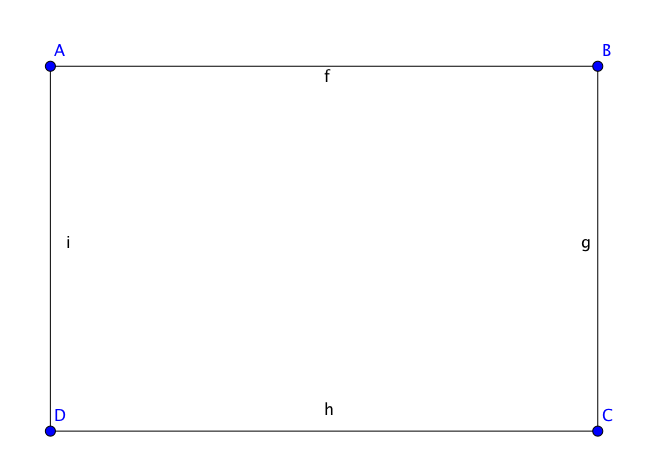
\includegraphics[width=\linewidth]{original_shape}
\caption{Original shape}\label{fig:mouse}
\end{subfigure}\hspace{20 mm}
\begin{subfigure}[b]{.4\linewidth}
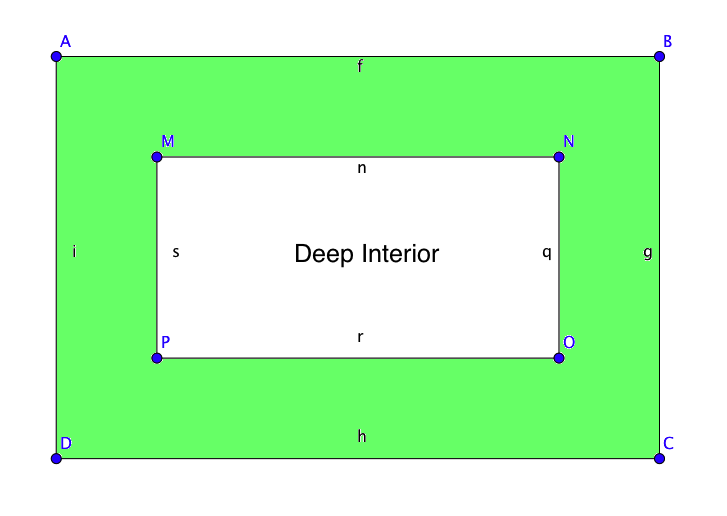
\includegraphics[width=\linewidth]{inner_boundary}
\caption{Inner set $A$ in green}\label{fig:gull}
\end{subfigure}

\begin{subfigure}[b]{.4\linewidth}
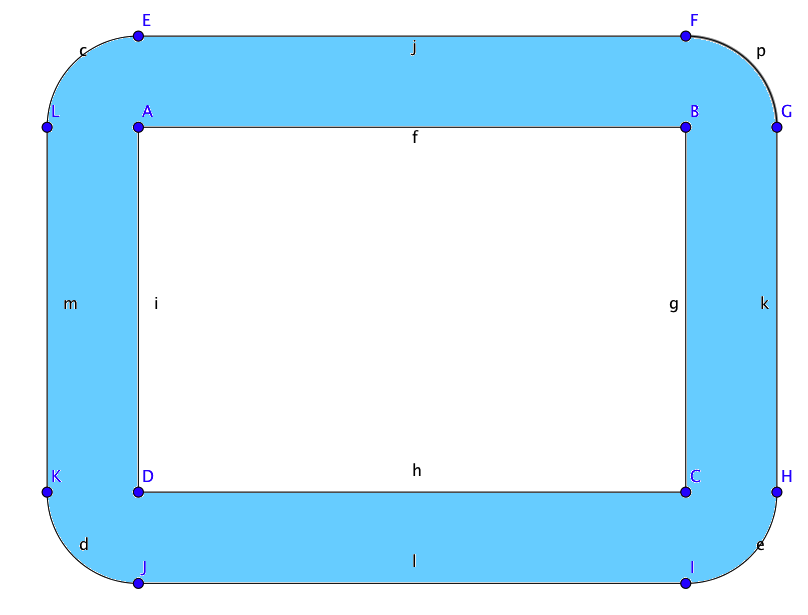
\includegraphics[width=\linewidth]{outer_boundary}
\caption{Outer set $B$ in blue}\label{fig:tiger}
\end{subfigure}\hspace{20 mm}
\caption{Illustration of inner and outer sets for approximate convex hull}
\label{fig:animals}
\end{figure}

\begin{lemma}
The boundary $U$ of the convex closure of $S$ must be contained in the union of $A$ and $B$.
\label{lem:sboundary}
\end{lemma}

\begin{proof}
First, we show that $U$ cannot intersect with the deep interior. To see this, suppose we choose the origin to be contained inside the deep interior (if the deep interior is empty then the claim is vacuously true). $S$ is an $\epsilon$-approximate convex hull of $P$ and $O \subseteq P$, so $S$ is an $\epsilon$-approximate convex hull of $O$. Then for all unit vectors $v$, |$\max_{o \in O} \langle o, v \rangle$ - $\max_{s \in S} \langle s, v \rangle| \leq \epsilon$. That is, in every direction, $U$ must be within distance $\epsilon$ from the boundary of the convex closure of $O$. But in every direction, the deep interior is greater than distance $\epsilon$ from the boundary of the convex closure of $O$.
\\

Next, we need to show that all points in the convex closure of $S$ are within distance $\epsilon$ from the convex closure of $O$. But this is true because $O$ is an $\epsilon$-approximate convex hull of $P$ and $S \subseteq P$, so $O$ is an $\epsilon$-approximate convex hull of $S$.
\end{proof}

By lemma~\ref{lem:sboundary}, since we delete all interior points in $S$ (lines 7 and 8), every point in the deep interior will be eventually discarded. Now, examine figure 2, which shows the top half of the original rectangle defined by $O$, along with corresponding parts of $A$ and $B$. Regions $C1, C2, E$ are part of the outer set $B$, and $I$ is part of the inner set $A$. In regions $C1$ and $C2$ we will select at most a constant number of points, because it is contained in a circle of radius $\epsilon$. There are OPT such regions. 
\\

In region $E$, we can use an argument similar to the 1D case to show that we will select, with high probability, at most $O(\log{n})$ points. This is because the height of $E$ is $\epsilon$. The idea is that we can view the line $AB$ as the $x$-axis, and consider the $x$-coordinate of each point in $O$. We will discard every new point in $E$ unless it has $x$-coordinate greater than all the current points we have seen in $E$, or $x$-coordinate lesser than all the current points we have seen in $E$. This reduces the problem to the 1D insertion only problem, so with probability $1-1/n^3$ we keep $O(\log{n})$ points.
\\

\begin{figure}
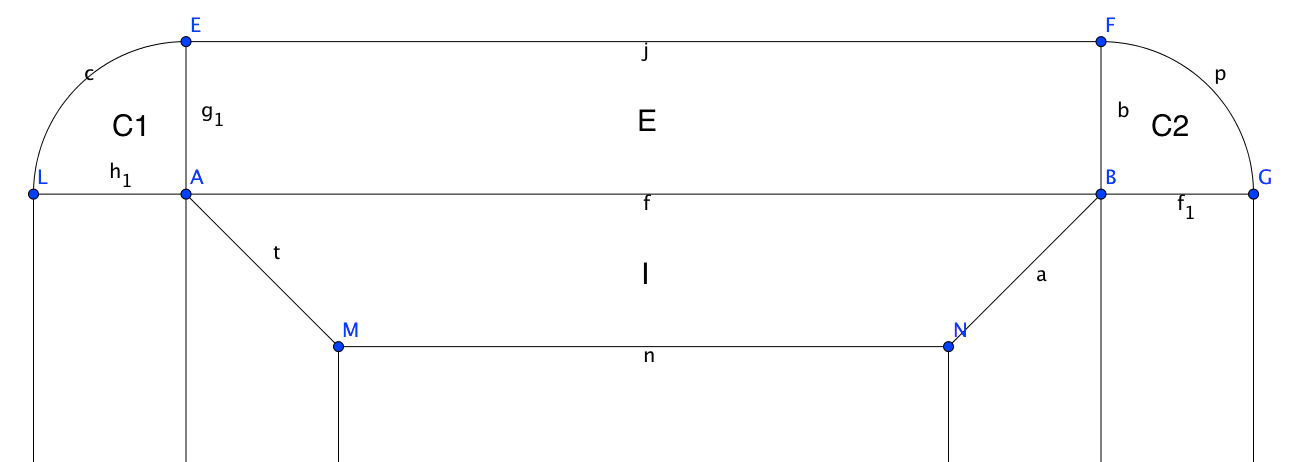
\includegraphics[width=\linewidth]{main_regions}
\caption{Important regions around approximate convex hull}\label{fig:tiger}
\end{figure}

The same argument applies to $I$. Note that there are OPT regions like $I$ and OPT regions like $E$, so by union bound, the total number of points we keep is $O(\mbox{OPT} \cdot \log{n})$ with high probability.
\end{proof}

Note that theorem~\ref{thm:2droaspace} gives us a high probability bound so:
\begin{enumerate}
\item Since ROA never keeps more than $n$ points (the entire set), we can use the high probability bound to show that the expected number of points ROA keeps is $O(\mbox{OPT}\log{n})$.
\item We can show that with high probability, when ROA has processed a prefix $P'$ containing the first $i$ out of $n$ points of $P$, ROA keeps an $\epsilon$-approximate convex hull of size $O(\mbox{OPT}(P', \epsilon)\log{n})$. Importantly, with high probability, this holds \emph{for all prefixes}, that is, throughout the entire stream.
\end{enumerate}

Unfortunately, this algorithm does not give good gaurantees in 3D. The 3D case reduces to the 2D intertion only case, where we run ROA without removing interior points. However, in the worst case we might end up choosing a large number of points.


\chapter{$\epsilon-\delta$ Hull Algorithms}

In this chapter we give an algorithm for a relaxation of $\epsilon$-approximate hulls, called $(\epsilon, \delta)$ hulls. Our results hold for arbitrary point sets $P \subseteq \mathbb{R}^d$.
\\

Intuitively, an $(\epsilon,\delta)$ hull of $P$ is within distance $\epsilon$ from the boundary of the convex closure of $P$ in at least $1-\delta$ directions. We begin by giving an equivalent definition for an $\epsilon$-approximate convex hull, and then define $(\epsilon,\delta)$ hulls.

\section{Definition of $(\epsilon, \delta)$ hull}

\begin{definition}
Given a vector $v$ and a point set $P$, we define the \textbf{directional extent} as
\[ \omega_v(P) = \max_{p \in P} p \cdot v \]
\label{def:dir_extent}
\end{definition}
\begin{definition}
If $p$ is a point we define $\omega_v(p) = p \cdot v = \omega_v(\{p\})$
\end{definition}

It is easy to see that if $S \subseteq P$ then for all $v$, $\omega_v(S) \leq \omega_v(P)$.

\begin{definition}
We say $S$ \textbf{maximizes} $P$ in $v$ if
\[ \omega_v(P) = \omega_v(S) \]
Note that as per definition~\ref{def:dir_extent}, $S$ can be either a single vector or a set of vectors.
\end{definition}

\begin{figure}[!htb]
\centering
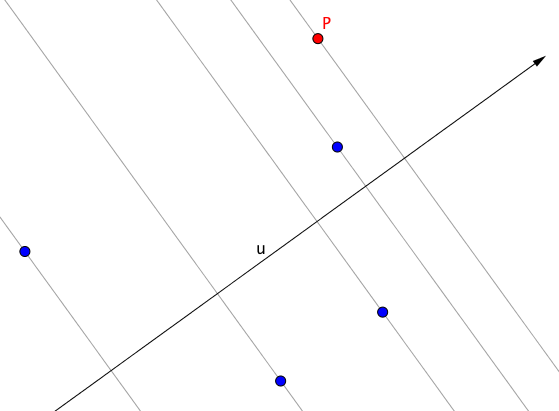
\includegraphics[width=0.5\linewidth]{maximal_point}
\caption{Point $p$ maximizes the set of points in direction $u$ because its projection onto $u$ is the highest.}
\label{fig:maximal_point}
\end{figure}

Figure~\ref{fig:maximal_point} shows a point $p$ that maximizes a set of points in direction $u$.

\begin{definition}
A \textbf{convex hull} is a subset $S \subseteq P$ such that $S$ maximizes $P$ in all (unit) directions $v$. 
\end{definition}

\begin{definition}
We say $S$ \textbf{$\epsilon$-maximizes} $P$ in direction $v$ if $v$ \emph{is a unit vector} and
\[ |\omega_v(P) - \omega_v(S)| \leq \epsilon \]
Note that as per definition~\ref{def:dir_extent}, $S$ can be either a single vector or a set of vectors.
\end{definition}

\begin{definition}
An \textbf{$\epsilon$-approximate convex hull} is a subset $S \subseteq P$ such that $S$ $\epsilon$-maximizes $P$ in all (unit) directions $v$. As before, OPT$(P, \epsilon)$ is the size of a smallest $\epsilon$-approximate convex hull.
\end{definition}

Intuitively, an $\epsilon$-approximate convex hull approximates the original point set in all directions. Coming up with a streaming algorithm that is competitive within a constant factor of OPT for this problem appears to be difficult. An interesting relaxation is to have a good approximation in \emph{most directions}. In the sections that follow, we will assume that the algorithm has access to OPT and sets $k = \mbox{OPT}$. In practice, we do not know OPT so we would simply set $k$ to be the largest value our computational resources permit. We would then have an $(\epsilon, \delta)$-approximation for all point sets where $\mbox{OPT} \leq k$. This is similar to the form of the lower bound we gave in theorem~\ref{thm:almostalwaysopt} in chapter~\ref{chapter:lower_bounds}.

\begin{definition}
An \textbf{$(\epsilon, \delta)$-hull} is the minimal sized set $S \subseteq P$ such that if we pick a vector $v$ uniformly at random from the surface of the unit sphere, $\mathcal{S}^{d-1}$, $S$ $\epsilon$-maximizes $P$ in direction $v$ with probability at least $1-\delta$, that is,
\[ \mbox{Pr}(|\omega_v(P) - \omega_v(S)| > \epsilon) \leq \delta \]
\end{definition}

Our goal is to come up with streaming algorithms for $(\epsilon, \delta)$-hulls that are competitive with OPT (the batch optimal for $\epsilon$-approximate convex hulls).

\section{Core Lemmas}

\begin{definition}
Define $E^S_s$ to be the set of all vectors $v$ in $\mathbb{R}^d$ (\emph{not just unit vectors}) such that $s$ maximizes $S$ in $v$, that is,
\[ E^S_s = \{ v \; | \; v \cdot s = \omega_v(S) \} \]
\end{definition}

\begin{figure}[!htb]
\centering
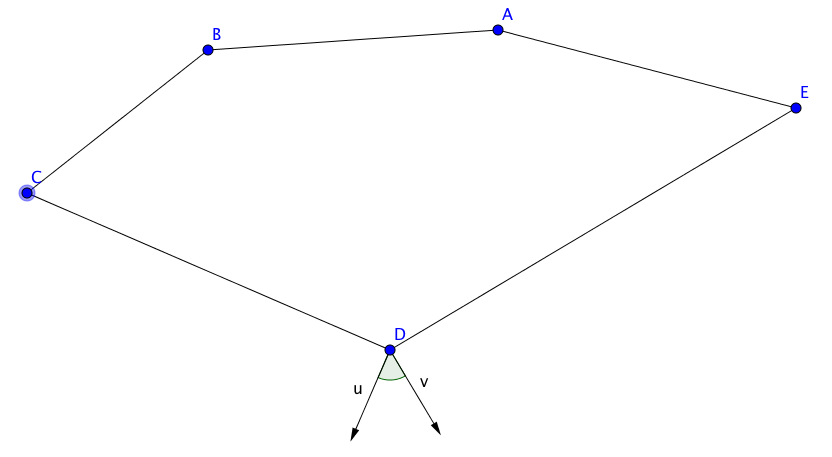
\includegraphics[width=0.7\linewidth]{maximizing_vector_range}
\caption{All vectors between $u$ and $v$ (not just unit vectors) are in $E_D^S$}
\label{fig:maximizing_vector_range}
\end{figure}

Figure~\ref{fig:maximizing_vector_range} shows a set of points $S$. All vectors between $u$ and $v$ (not just unit vectors), in the range indicated by the angle, are in $E_D^S$. Note that $u$ is perpendicular to line segment $CD$ and $v$ is perpendicular to line segment $DE$. Only points $s \in S$ that lie on the boundary of the convex closure of $S$ have non-empty $E_s^S$.

\begin{lemma}[$\epsilon$-Maximization Lemma] Suppose $S \subseteq P$ is an $\epsilon$-approximate convex hull of $P$, and fix $s \in S$. Then $s$ $\epsilon$-maximizes P for all unit vectors $v \in E^S_s$.
\end{lemma}

\begin{proof}
This is because for all unit vectors $v$, $|\omega_v(S) - \omega_v(P)| \leq \epsilon$ and for all vectors $v \in E^S_s$, $v \cdot s = \omega_v(S)$, so for all unit vectors $v \in E^S_s$, both properties hold.
\end{proof}

\begin{lemma}[Covering Lemma] For all vectors $v \in \mathbb{R}^d$,
\[ v \in \bigcup_{s \in S} E^S_s \]
\end{lemma}

\begin{proof}
Given any vector $v$, set $s = \displaystyle\argmax_{s' \in S} s' \cdot v$. Then $v \in E^S_s$.
\end{proof}

\begin{lemma} [Conic Lemma] $E^S_s$ is a cone, that is,
\begin{enumerate}
\item $0 \in E^S_s$
\item If $v \in E^S_s$ and $\alpha \in \mathbb{R^+}$ then $\alpha v \in E^S_s$.
\item If $v, w \in E^S_s$ then $v + w \in E^S_s$.
\end{enumerate}
\end{lemma}

\begin{proof} We prove each item,
\begin{enumerate}
\item $0 \cdot s = \max_{s' \in S} 0 \cdot s' = 0$
\item $(\alpha v) \cdot s = \alpha (v \cdot s) = \alpha (\max_{s' \in S} v \cdot s') = \max_{s' \in S} (\alpha v) \cdot s'$
\item $(v + w) \cdot s = (v \cdot s) + (w \cdot s) = \max_{s' \in S} v \cdot s' + \max_{s' \in S} w \cdot s' \geq \max_{s' \in S} (v + w) \cdot s'$
\end{enumerate}
\end{proof}

\begin{lemma} [Cutting Lemma] Given any 2 points $a \neq b \in \mathbb{R}^d$, let $H = \{v \; | \; v \cdot a \geq v \cdot b\}$. Then $H$ is a closed halfspace cutting through the origin.
\end{lemma}

\begin{proof}
Writing this in another way, $H = \{v \; | \; v \cdot (a - b) \geq 0\}$, which, if $a-b \neq 0$, is precisely the equation of a closed halfspace. The plane defining the boundary of the halfspace is defined by $P = \{v \; | \; v \cdot (a - b) = 0\}$ (that is, the set of all vectors perpendicular to $a-b$) which cuts through the origin.
\end{proof}

\begin{lemma} [Bounded Maximization Lemma] Suppose $S$ has at least 2 distinct points. Then if $s \in S$, $E^S_s$ is contained inside a closed halfspace passing through the origin.
\end{lemma}

\begin{proof}
Choose $s' \in S$ with $s' \neq s$. Then, let $H = \{v \; | \; v \cdot s \geq v \cdot s'\}$. $E^S_s \subseteq H$ but by the cutting lemma, $H$ is a closed halfspace passing through the origin.
\end{proof}

\section{2D-Algorithm}

We give a deterministic algorithm that stores $O(\frac{k}{\delta})$ points and gives us an $(\epsilon, \delta)$-hull of a point set $P$, where $k$ is the batch optimal for the $\epsilon$-approximate convex hull of $P$.
\\

\begin{figure}[!htb]
\centering
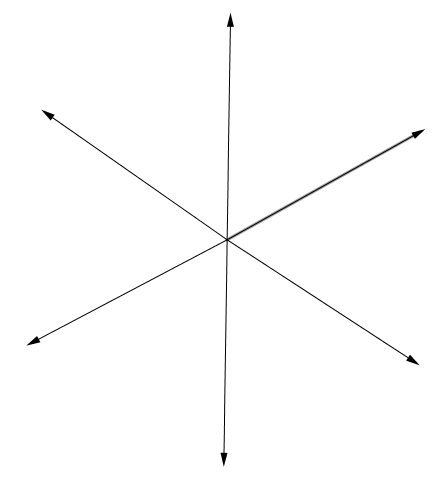
\includegraphics[width=0.3\linewidth]{equally_spaced_directions}
\caption{6 equally separated directions.}
\label{fig:equally_spaced_directions}
\end{figure}

Choose $O(\frac{k}{\delta})$ equally separated unit vectors (like in figure~\ref{fig:equally_spaced_directions}) on the boundary of the unit circle. Going counter-clockwise by angle, the angle formed by any 2 consecutive vectors will be less than $\frac{2\pi\delta}{k}$. For each chosen vector $v$ we store the point $p \in P$ s.t. $p \cdot v = \omega_v(P)$ ($p$ maximizes $P$ in $v$). This can be done in streaming - for a vector $v$, we keep an incoming point $p$ iff $v \cdot p$ is greater than $v \cdot p'$ for the point $p'$ we currently stored in direction $v$ (or if we have not stored any point for direction $v$). Call the set of points our algorithm chooses $T$.

\begin{theorem}
$T$ is an $(\epsilon, \delta)$-hull of $P$.
\end{theorem}

\begin{proof}
WLOG suppose that $P$ has at least 2 distinct points (otherwise we can trivially solve the problem by storing the only point in $P$). Consider an optimal $\epsilon$-approximate convex hull $S \subseteq P$. WLOG suppose that S contains at least 2 points (otherwise we can simply add some point in $P$ to $S$ and our bounds will only change by a constant factor). 
\\

\textbf{Partitioning}: Pick a vector $v$ uniformly at random on the boundary of the unit circle. By the covering lemma, $v \in E^S_s$ for some $s \in S$. Fix $s \in S$. It suffices to show the probability that $v \in E^S_s$ and $T$ does not $\epsilon$-maximize $P$ in direction $v$ is $\leq \frac{\delta}{k}$. Then, since there are $k$ choices for $s$, the probability $T$ does not $\epsilon$-approximate $P$ is $\leq k\frac{\delta}{k} = \delta$.
\\

\textbf{Angular setup}: Fix $s \in S$. $S$ has at least 2 distinct points, so by the cutting lemma, $E^S_s$ is contained in a half-space. So we can rotate space such that $E^S_s$ does not contain the positive x axis. We measure angles counter-clockwise from the positive x-axis. From the conic lemma, we know that $E^S_s$ is the set of all vectors with angles between $\theta_a$ and $\theta_b$ with $\theta_a < \theta_b$. Out of the $O(\frac{k}{\delta})$ vectors we chose, consider the subset of vectors that are in $E^S_s$. Call them $v_1, v_2, ..., v_m$ and suppose they have corresponding angles $\theta_1 < \theta_2 < ... < \theta_m$. We also have that $\theta_a \leq \theta_1$ and $\theta_m \leq \theta_b$.
\\

\begin{lemma}
Consider some $v_i$. We choose a point $p_i$ s.t. $p_i \cdot v_i = \omega_{v_i}(P)$ (that is, $p_i$ is maximal in direction $v_i$). We will show that $p_i$ $\epsilon$-maximizes either all unit vectors with angles in the range $[\theta_a, \theta_i]$ or in $[\theta_i, \theta_b]$
\end{lemma}

\begin{proof}
If $p_i = s$, then $p_i$ $\epsilon$-maximizes all unit directions in $E^S_s$, so we are done. Otherwise, suppose $p_i \neq s$. By the cutting lemma, there exists a closed half-space $H$ passing through the origin, such that $p \cdot v \geq s \cdot v$ iff $v \in H$. By the $\epsilon$-maximization lemma, for all unit vectors $v \in E_s$, $0 \leq \omega_v(P) - s \cdot v \leq \epsilon$. This implies that for all unit vectors $v \in E_s \cap H$, $0 \leq \omega_v(P) - p \cdot v \leq \omega_v(P) - s \cdot v \leq \epsilon$. In other words, $p$ $\epsilon$-maximizes all unit vectors $v \in E_s \cap H$.
\\

Since $E_s$ is itself contained in some halfspace passing through the origin, $E_s \cap H$ is either the set of vectors with angles in range $[\theta, \theta_b]$ or in range $[\theta_a, \theta]$. We note that $v_i \in E_s \cap H$ and has angle $\theta_i$, so in either case the range contains $\theta_i$. This proves the lemma.
\end{proof}

We say that $v_i$ is \emph{down} if $p_i$ $\epsilon$-maximizes $P$ in all directions with angles in the range $[\theta_a, \theta_i]$ and \emph{up} if $p_i$ $\epsilon$-maximizes $P$ in all directions with angles in the range $[\theta_i, \theta_b]$. If $v_1$ is up, then $p_1$ $\epsilon$-maximizes $P$ in all directions with angles in $[\theta_1, \theta_b]$. The angle between $\theta_a$ and $\theta_1$ is $\leq \frac{2\pi\delta}{k}$ because we chose vectors that were $\frac{2\pi\delta}{k}$ apart, so we are done. A similar argument applies if $v_m$ is down, and if $m = 0$ (we did not choose any vectors between $\theta_a$ and $\theta_b$. Otherwise, we consider the smallest $i$ s.t. $v_i$ is down but $v_{i+1}$ is up. Then, $p_i$ $\epsilon$-maximizes $P$ in all directions with angles in $[\theta_a, \theta_i]$ and $p_{i+1}$ $\epsilon$-maximizes $P$ in all directions with angles in $[\theta_{i+1}, \theta_b]$. We might not $\epsilon$-maximize $P$ in directions with angles in the range $[\theta_i, \theta_{i+1}]$, but this angle is $\leq \frac{2\pi\delta}{k}$.
\end{proof}


\section{Generalizing to higher dimensions}

\subsection{Algorithm}

Suppose we fix the dimension $d$. We give a randomized algorithm that uses $n$ points and with probability at least $1-p$ gives us an $(\epsilon, \delta)$-hull of a point set $P$, where $k$ is the batch optimal for the $\epsilon$-approximate convex hull of $P$ and $n$ satisfies,
\[ n \in O\left(\frac{k^2}{\delta^2}\left(\log{k} + \log{\frac{1}{\delta} + \log{\frac{1}{p}} }\right)\right) \]

Note that the given complexity hides the dependency on $d$, so the actual complexity will be $O(f(d) \frac{k^2}{\delta^2}\left(\log{k} + \log{\frac{1}{\delta} + \log{\frac{1}{p}} }\right))$ for some function $f : \mathbb{N} \to \mathbb{N}$
\\

The algorithm is simple: Choose $n$ random vectors on the unit sphere. For each chosen vector $v$ we store the point $p$ that maximizes $P$ in direction $v$, that is, $p \cdot v = \omega_v(P)$. As in the 2D algorithm, this can be done in streaming.

\subsection{3D Proof Outline}

As before, WLOG suppose that $P$ has at least 2 distinct points (otherwise we can trivially solve the problem by storing the only point in $P$). Consider an optimal $\epsilon$-approximate convex hull $S \subseteq P$. WLOG suppose that S contains at least 2 points (otherwise we can simply add some point in $P$ to $S$ and our bounds will only change by a constant factor). 
\\

\textbf{Constructing small triangular cones}: A triangular cone is a cone defined by the non-negative sums of 3 vectors. First, we choose $c$ ``small" triangular cones, where $c$ is a large constant. Consider a triangle cone defined by unit vectors $v_1, v_2, v_3$. More precisely, we choose the cones so that $\max(|v_1 - v_2|_2, |v_2 - v_3|_2, |v_1 - v_3|_2) < 0.01$. We choose the cones so that they are disjoint, and they span $\mathbb{R}^d$, that is, every vector is in some cone.. Intuitively, we can construct these cones as follows: we start out with $2^d$ triangular cones that span $\mathbb{R}^d$. Then we can keep making the cones smaller (we can select a vector in the middle of each cone to split it up into 3 cones) until the cones satisfy the required condition. The number of cones is some function of the dimension $d$.
\\

\textbf{Cutting cones}: Consider a cone $C \cap E^S_s$. Intuitively, we are going to show that each time we choose a vector $v$, we cut away part of $C \cap E^S_s$ (for the part we cut off, we have an $\epsilon$-maximization). Consider each unit vector $v$ we choose in cone $C \cap E^S_s$, and corresponding point $p$ that maximizes $P$ in $v$. If $p = s$, then $p$ $\epsilon$-maximizes the whole cone $E^S_s$ so we are done. Otherwise, by the cutting lemma, there exists a closed half-space $H$ passing through the origin, such that $p \cdot v' \geq s \cdot v'$ iff $v' \in H$. As in the 2D proof, $p$ then $\epsilon$-maximizes all vectors in $E^S_s \cap H$ and therefore in $C \cap E^S_s \cap H$. So the region of $C \cap E^S_s$ that we might not have $\epsilon$-maximized is $C \cap E^S_s \cap H^c$. $C \cap E^S_s \cap H^c \subseteq C \cap E^S_s \cap (H^c \cup \{0\})$. $(H^c \cup \{0\})$ is a cone, and the intersection of cones is a cone, so  $C \cap E^S_s \cap (H^c \cup \{0\})$ is also a cone. Note that $v \in H$ and $v \neq 0$, so $v \not\in C \cap E^S_s \cap (H^c \cup \{0\})$.
\\

\textbf{Projection}: After choosing many vectors $v \in C \cap E^S_s$, we end up with a cone $C' \subseteq C \cap E^S_s$ where $C'$ does not contain any of the selected vectors $v$. We want to show that the area of $C' \cap \mathbb {S}^2$ is less than $\frac{\delta}{ck}$ fraction of the unit sphere's area. Then, adding over the $ck$ cones, the proportion of unit vectors we don't $\epsilon$-maximize in $P$ is at most $\delta$. The main trick will be to project this into a 2-dimensional problem. Suppose that (triangular) cone $C$ was defined by vectors $v_1, v_2, v_3$. Consider the plane $P$ containing the endpoints of $v_1, v_2, v_3$. We project $C \cap E^S_s \cap \mathbb {S}^2$ onto $P$, and similarly project all unit vectors we chose that are in $C \cap E^S_s \cap \mathbb {S}^2$ onto $P$, and project $C' \cap \mathbb {S}^2$ onto $P$. 
\\

\textbf{Reduced problem}: This gives us a simpler problem. Suppose we have convex polygon $C$ with area $A$, where we choose points in $C$ from a nearly uniform distribution $\pi$. More formally, the ratio between the max and min of the PDF of $\pi$ is at most 2. Call a convex polygon \emph{respectful} if it does not contain any selected points. How many points do we need to choose so that with high probability, all respectful convex polygons contained in $C$ must have area $\leq \frac{\delta}{k}$? The reason this reduction holds is because we chose cone $C$ to be small, so $C \cap \mathbb {S}^2$ is quite flat. In particular, if we rotate space so that plane $P$ is perpendicular to the $z$ axis, the norm of the gradient of $C \cap \mathbb {S}^2$ is bounded by 2. So when a set of measure $v$ in $C \cap E^S_s \cap \mathbb {S}^2$ is projected to $P$ it has measure between $\frac{v}{2}$ and $v$.

\begin{lemma}
Given a convex polygon $C$, there exists 3 points in $C$ such that the triangle formed between them has area at least $\frac{1}{4}$ the area of $C$.
\label{lemma:convex_approx}
\end{lemma}

\begin{lemma}
The pdf of $\pi$ must be between $\frac{1}{2A}$ and $\frac{2}{A}$ everywhere.
\end{lemma}

\textbf{Uniform Bound Outline} Let $T$ be the set of triangles contained in polygon $C$ with area $\geq \frac{\delta}{4ck}$.  Given $t \in T$, let $P(t)$ denote the probability that a point selected from $\pi$ lies in $t$. Since $\pi$ is almost uniform, $P(t) \geq \frac{\delta}{8Ack}$. We will use uniform bounds and VC dimension, to show that if we select enough points in $C$ then with high probability \emph{every} triangle in $T$ will contain a point. This is sufficient to solve the problem: consider arbitrary convex polygon $G$ contained in $C$ with area $\geq \frac{\delta}{ck}$. By lemma~\ref{lemma:convex_approx}, it contains a triangle of area $\geq \frac{\delta}{4ck}$. But all such triangles contain a point, so $G$ contains a point. Therefore every convex polygon in $C$ that does not contain a point must have area $< \frac{\delta}{ck}$.
\\

\textbf{Sampling Process} Select $n$ points in $C$ from distribution $\pi$. For $t \in T$, let $C_n(t)$ be the number of selected points that lie in $t$, and let $P_n(t)$ be $\frac{C_n(t)}{n}$. Intuitively, we are estimating the cumulative density of $\pi$ in a region by sampling points and computing the proportion of points that fall in the region. Suppose that for all $t \in T$, $|P_n(t) - P(t)| < \frac{\delta}{8Ack}$ (this means that $P_n$ approximates $P$ well). Then, for all $t$, since $P(t) \geq \frac{\delta}{8Ack}$, $P_n(t) > 0$. This means that every triangle $t \in T$ contains a point.
\\

\textbf{VC Dimension} We want to show that with probability at least $1-\frac{p}{2ck}$, $\sup_{t \in T} |P_n(t) - P(t)| < \frac{\delta}{8Ack}$. The VC dimension of $T$ is 7. Letting $\epsilon = \frac{\delta}{8Ack}$, we apply a VC-dimension based uniform bound to get that,
\[ P(\sup_{t \in T} |P_n(t) - P(t)| > \epsilon) \leq 8(n+1)^7 e^{-n\epsilon^2/32} \]

We set $n \in O(\frac{(Ack)^2}{\delta^2} (\log{\frac{Ack}{\delta}} + \log{\frac{k}{p}}))$.
\\

\textbf{Finishing up}: Consider a cone $C \cap E^S_s$. Suppose that the intersection $C \cap E^S_s \cap \mathbb {S}^2$ has area $A$. The projection has area $\leq A$, so it suffices to choose $n \in O(\frac{A^2k^2}{\delta^2} (\log{\frac{Ak}{\delta}} + \log{\frac{k}{p}}))$ unit vectors in $C \cap E^S_s \cap \mathbb {S}^2$. When we choose a unit vector at random, it lies in $C \cap E^S_s \cap \mathbb {S}^2$ with probability $c = \frac{A}{4\pi}$. We want to choose $m$ points, so that with probability at least $1-\frac{p}{2ck}$ we have $n$ points inside the cone. From a standard Chernoff bound argument, $m \in O(\frac{n}{c}(\log{n} + \log{\frac{k}{p}} ))$ works. Simplifying, this becomes,
\begin{align*}
m &= O\left(\left[\left(\frac{A^2k^2}{\delta^2} \left(\log{\frac{Ak}{\delta}} + \log{\frac{k}{p}}\right)\right)\left(\frac{4\pi}{A}\right)\right]\left[ \log{n} + \log{\frac{k}{p}} \right]\right) \\
&= O\left( \left[\left(\frac{Ak^2}{\delta^2} \left(\log{\frac{Ak}{\delta}} + \log{\frac{k}{p}}\right)\right)\right]\left[ \log{n} + \log{\frac{k}{p}} \right] \right)
\end{align*}

We note that $A \leq 4\pi$. Furthermore, $\log{n}$ actually simplifies to
\[ O(\log{\frac{k}{\delta}} + \log(\log{\frac{k}{\delta}} + \log{\frac{k}{p}})) \subseteq O(\log{\frac{k}{\delta}} + \log{\frac{k}{p}}) \]

So in the worst case $m$ reduces to
\[ m \in O\left(\frac{k^2}{\delta^2}\left(\log{k} + \log{\frac{1}{\delta} + \log{\frac{1}{p}} }\right)\right) \]
We can apply union bounds over the cones to get a $\leq p$ chance of failure.

\subsection{Arbitrary Dimension Proof Sketch}

A few parts of the proof need to be modified to deal with higher dimensions.
\begin{enumerate}
\item The section where we construct small triangular cones. In $d$ dimensional space, the cones will be defined by $d$ vectors (so the endpoints of the vectors form a simplex instead of a triangle) such that the pairwise distance between any 2 vectors is at most 0.1. The construction is as described above.
\item We need to modify lemma~\ref{lemma:convex_approx}. In particular instead of triangles, we will use ellipsoids. Given any convex body $C$ with area $A$, there exists an ellipsoid contained inside $C$ with area at least $A/d^d$~\cite{geom_approx_algs}.
\item The VC dimension of an ellipsoid in $d$-dimensional space is $O(d^2)$ (we used the factor that the VC dimension of a triangle in 2D space is 7).
\end{enumerate}
The rest of the proof outline is the same, so this gives us the desired result.

\chapter{Discussion}
The aim of this undergraduate thesis was to examine streaming algorithms for $\epsilon$-approximate convex hulls in relation to OPT. We proved some lower bounds for this empirically difficult problem, which should guide future research into related problems. We also devised and proved algorithms for 2 relaxations of the problem: when the points are in 2D and come in a random order, and for $(\epsilon,\delta)$-hulls.
\\

There is lots of exciting work to be done on this topic. We list some interesting research directions.
\begin{enumerate}
\item Examine the connections between $\epsilon$-approximate convex hulls, $(\epsilon, \delta)$-hulls, and matrix factorization in more detail, in particular with experiments to check if the factorizations produced by finding an approximate convex hull are meaningful.
\item Our random order algorithm does not work in 3D (or higher dimensions). Come up with an algorithm that works in higher dimensions, assuming the points come in random order. Alternatively, come up with a lower bound when the points come in random order.
\item Our algorithm for $(\epsilon, \delta)$-hulls works in arbitrary dimensions, however it does not scale well with $d$. Our algorithm can only be used when the dimension is low. In fact, all provable streaming algorithms for $\epsilon$-approximate convex hulls, or related problems, do not scale well with $d$. Come up with algorithms for $(\epsilon, \delta)$-hulls, or other interesting relaxations, that work in high dimensions.
\item We do not have any lower bounds for the 2D $\epsilon$-approximate convex hull problem. We were not able to devise an algorithm that is competitive with OPT for this problem after extensive effort, however there might exist a clever algorithm that solves this problem. Alternatively, we could try proving lower bounds for the 2D problem.
\item Coming up with algorithms for $\epsilon$-kernels that are competitive with the optimally sized $\epsilon$-kernel of a point set. While $\epsilon$-approximate convex hulls play a key role in finding $\epsilon$-kernels, an algorithm that is competitive with OPT for $\epsilon$-approximate convex hulls might not immediately give an algorithm that is competitive with OPT for $\epsilon$-kernels.
\end{enumerate} 

\chapter*{Appendix A: Experiments with NMF}

The MNIST database contains labeled images of handwritten digits~\cite{lecun}. Each image is represented by a 28-by-28 grid of black-white intensity values. The training set has 60,000 samples and the testing set has 10,000 samples. A variety of algorithms have been tested for supervised classification on the MNIST database.
\\

Our approach for using NMF for supervised classification is similar to Lee and Seung's ~\cite{Lee97unsupervisedlearning}. For the training set, we separate the images which are associated with each digit (to get 10 sets of images). We find the NMF for each of these separated sets. Then for each test image, we try to reconstruct it using the NMF topic matrix for each digit. We output the digit whose topic matrix best reconstructs the image. Intuitively, we are finding the parts that comprise each handwritten digit, and given a new image we are finding the parts that best represent the new image.
\\

We normalize each image before running the algorithms so that each image has Euclidean norm 1. We test a variety of different NMF algorithms. We first use two-fold cross-validation on the training set to find good sizes for the NMF topics matrices. In this stage we randomly split the training set into two parts $A$ and $B$. We train the NMF algorithm on $A$ and check its accuracy on $B$ for various sizes of topic matrices. We repeat the cross-validation process 5 times for each NMF algorithm and each topic matrix size in (10, 20, 30, ..., 90). We did not touch the test set in this stage so that the runs on the test set would be independent of the optimization process and could be used to get generalization guarantees for them.
\\

In the next stage, we trained the NMF algorithms on the training set, and used them to classify images in the test set. Let the topic matrix size be $t$. We tested 4 different algorithms:
\\

\textbf{Matlab NMF} Uses the Matlab library functions for (non-sparse, non-convex) non-negative matrix factorization and quadratic programming for reconstructing a test image from the NMF topic matrix.
\\

\textbf{Simple Hull} We pick the first $t$ samples of each digit as our topics. Given a new image, we used convex quadratic programming to find the distance of the image to the convex hull of the topic matrix. The digit with the lowest distance is selected.
\\

\textbf{Gonz Hull} We use a variant of the Gonzales algorithm to select the $t$ topics~\cite{blum-peled}. In the Gonzales algorithm, at each step we look for the point that is farthest away from the current convex hull. This is exceedingly slow (at least on the order of days) on the MNIST database because there are up to 50,000$^2$ calls to a quadratic programming subroutine. Instead, in each iteration we sample 15 random points and choose the point (out of the 15) that is farthest from the current convex hull. The reconstruction process is the same as in the Simple Hull method.
\\

\textbf{Push Gonz Hull} This is an extension we propose to the Gonzales algorithm for spherical convex hull NMF. In the Gonzales algorithm, after selecting each point, we `push' the point to the boundary of the non-negative region of the unit sphere.
\\

\begin{table}[h!]
\centering
\begin{tabular}{ |c|c|c|c| } 
 \hline
  Method & NMF Size & Error (\%) \\ 
 \hline
 Matlab NMF & 60 & 8.6 \\ 
 \hline
 Simple Hull & 60 & 10.7 \\ 
 \hline
  Gonz Hull & 60 & 9.7 \\ 
 \hline
  Push Gonz Hull & 60 & 9.4 \\ 
 \hline
  Matlab NMF & 100 & 9.1 \\ 
 \hline
 Simple Hull & 100 & 10.0 \\ 
 \hline
  Gonz Hull & 100 & 6.6 \\ 
 \hline
  Push Gonz Hull & 100 & 7.2 \\ 
 \hline
  Simple Hull & 5000 & 2.1 \\ 
 \hline
\end{tabular}
\caption{Supervised classification error of NMF algorithms}
\label{tab:main_results_table}
\end{table}

The results of our tests are shown in table~\ref{tab:main_results_table}. We used the first 2000 of the 10,000 samples in the testing set. Given the number of samples we used, the 95\% standard error of the difference in errors (which can be used when making comparisons across different methods) was 2\%. 
\\

Besides performing better than regular NMF, the simple hull method with a topic matrix size of 5,000 performed better than K-nearest neighbors, 2 layered neural nets, 3 layered neural nets~\cite{lecun}, and boosted stumps~\cite{kegl}. Note that the performance of Matlab's NMF peaked at a topic matrix of size 60, and performed badly on large sizes since it overfit the data, so the comparison between the Simple Hull and Matlab NMF method is fair even though the topic sizes are different.
\\

The convex NMF algorithms outperformed the regular NMF algorithm across sizes, which provides some validation for our theoretical models. Gonz Hull did better than our Push Gonz Hull which suggests that the algorithm we developed did not accurately capture the region represented by the digits but overextended itself to a larger region. However, the following table shows the classification error rate of the algorithms for smaller topic matrices. In this experiment, the first 5000 of the 60,000 training samples were used.

\begin{table}[h!]
\centering
\begin{tabular}{ |c|c|c|c| } 
 \hline
   Method/Size & 10 & 20 \\ 
 \hline
 Matlab NMF & 11.1\% & 9.5\% \\ 
 \hline
 Simple Hull & 30.1\% & 21.4\% \\ 
 \hline
  Gonz Hull & 24.2\% & 15.5\% \\ 
 \hline
  Push Gonz Hull & 23.2\% & 14.6\% \\ 
 \hline
\end{tabular}
\caption{Supervised classification error of NMF algorithms}
\label{tab:smaller_results}
\end{table}

For smaller topic matrices (shown in table~\ref{tab:smaller_results}), Push Gonz Hull does better than Gonz Hull. Although the difference in error rates is not statistically significant, it suggests that Push Gonz Hull might perform well on smaller training sets and when we want to use a small number of topics. More experiments should be done to verify this conjecture. The advantage of having a smaller topic matrix is that training and testing are significantly faster. Training and testing for a topic matrix 5 times smaller was at least 10 times faster in our (crude) initial experiments.

\chapter*{Appendix B: Collaboration Details}

This work was done in collaboration with Lin Yang, Harry Lang, and Vladimir Braverman. Since Lin, Harry, and Vova were external collaborators, I will briefly document the benefits I received from this external collaboration. 

\begin{enumerate}
\item Working with such wonderful collaborators was really useful for my research. Lin and Harry read up drafts of parts of this thesis that I sent them, checked my proofs, and gave me valuable feedback. We also bounced ideas off each other fairly often, and talked about papers we read.
\item The idea of working on streaming algorithms competitive with OPT was not mine.
\item It was Lin's idea to work on $(\epsilon, \delta)$-hulls when $\epsilon$-approximate convex hulls were difficult to deal with.
\item Lin came up with an initial randomized 2D algorithm for $(\epsilon, \delta)$-hulls that used $O(klogk)$ points, where $k$ is OPT$(P, \epsilon)$, and gives a $(\sqrt{\epsilon}, 1/2)$-hull
\item I suggested the deterministic 2D algorithm that uses $O(k/\delta)$ points and gives an $(\epsilon, \delta)$-hull. However, my original proof was more complicated, and Lin suggested a really clever idea for a simpler proof, which I used in the writeup.
\item I suggested and proved the higher dimensional algorithm, but used Lin's clever idea in part of my proof for the higher dimensional algorithm.
\item Note that all writing in this document is mine.
\end{enumerate}

Of course, Avrim provided invaluable advice throughout the course of this research.

% We recommend abbrvnat bibliography style.

\bibliographystyle{alpha}

% The bibliography should be embedded for final submission.

\bibliography{references}


\end{document}